\chapter{Differentialrechnung auf $\R$}
\section{Differential (Ableitung), Elementare Eigenschaften}
\begin{definition}{5.1}
Sei $f:\Omega\to\R$, $\Omega\subset\R$, und $x_0\in\Omega$
\begin{enumerate}
\item $f$ heisst differenzierbar an der Stelle $x_0$, falls
\[\lim_{\substack{x \to {x_0} \\ x\not  = {x_0}}}{\frac{f\left( x \right) - f\left( {{x_0}} \right)}{{x - {x_0}}}}\]
existiert. Dieser Grenzwert wird dann mit $f'\left( x_0\right)$ oder $\frac{df}{dx}\left( x_0\right)$ bezeichnet. Die Zahl $f'\left( x_0\right)$ heisst die Ableitung oder das Differential von $f$ an der Stelle $x_0$.
\item $f$ heisst in $\Omega$ differenzierbar, falls sie an jeder Stelle $x_0\in\Omega$ differenzierbar ist. In diesem Fall, nennt sich die Funktion $x\to f'(x)$ Ableitung von $f$.
\end{enumerate}
\end{definition}
\subsubsection*{Bemerkung 5.2}
In der Definition 5.1 verlangen wir also, dass für jede in $\Omega \backslash\{ x_0\}$ enthaltene Folge $\left( x_n\right)_{n\geq 1}$ mit Grenzwert $x_0$, der Limes
\[\mathop {\lim }\limits_{n \to \infty} \frac{{f\left( {x_n} \right) - f\left( {{x_0}} \right)}}{{x_n-x_0}} = 0\]
\subsubsection*{Bemerkung 5.3}
Sei $f$ differenzierbar in $x_0$
\begin{center}
\begin{tikzpicture}[scale=0.7]
\draw[->](-0.5,0) -- (6,0);
\draw[->](0,-0.5) -- (0,6);
\draw [in=-111, out=9] (0,1) to (5,5);
\draw[fill=black] (2.5,1.86) circle (0.05);
\draw[fill=black] (4.5,3.95) circle (0.05);
\draw (2.5,1.86) -- (4.5,3.95);
\draw[dashed] (2.5,1.86) -- (2.5,0) node[anchor=north] {$x_0$};
\draw[dashed] (4.5,3.95) -- (4.5,0) node[anchor=north] {$x$};
\draw[dashed] (2.5,1.86) -- (0,1.86) node[anchor=east] {$f\left(x_0\right)$};
\draw[dashed] (4.5,3.95) -- (0,3.95) node[anchor=east] {$f(x)$};
\end{tikzpicture}
\end{center}

Dann ist \[\frac{{f\left( x \right) - f\left( {{x_0}} \right)}}{{x - {x_0}}}\] die Steigung der Geraden durch die Punkte $\left( x_0,f\left( x_0\right) \right)$ und $\left( x,f\left( x\right) \right)$.\\

Geometrisch ist also $f'\left( x_0\right)$ die Steigung der Tangenten am Graphen von $f$ im Punkt $\left( x_0,f\left( x_0\right) \right)$. Diese Tangente hat die Gleichung
\[T(x) = f'\left( {{x_0}} \right)\left( {x - {x_0}} \right) + f\left( {{x_0}} \right)\]
Sei
\[f\left( x \right)= f'\left( {{x_0}} \right)\left( {x - {x_0}} \right) + f\left( {{x_0}} \right) + {R_{{x_0}}}\left( x \right) = T\left( x \right) + {R_{{x_0}}}\left( x \right)\]
\[ \Rightarrow \frac{{f\left( x \right) - f\left( {{x_0}} \right)}}{{x - {x_0}}} = \frac{{f'\left( {{x_0}} \right)\left( {x - {x_0}} \right)}}{{x - {x_0}}} + \frac{{R\left( x \right)}}{{x - {x_0}}}\]
Dann folgt
\[ \lim_{\substack{x \to {x_0} \\ x\not  = {x_0}}}{\frac{{R\left( x \right)}}{x - {x_0}}} = 0\]
Die lineare Funktion $f\left( {{x_0}} \right) + f'\left( {{x_0}} \right)\left( {x - {x_0}} \right)$ stellt eine gute Approximation der Funktion $f(x)$ dar:\\

\noindent Es gilt
\[ f \left( x \right) = f \left( {x_0} \right) + f' \left( {x_0} \right) \left( {x - {x_0}} \right) + {R_{x_0}}\left( x \right)\]
mit
\[\lim_{x \to {x_0}} \frac{R\left( x \right)}{x - {x_0}} = 0\]
\begin{center}
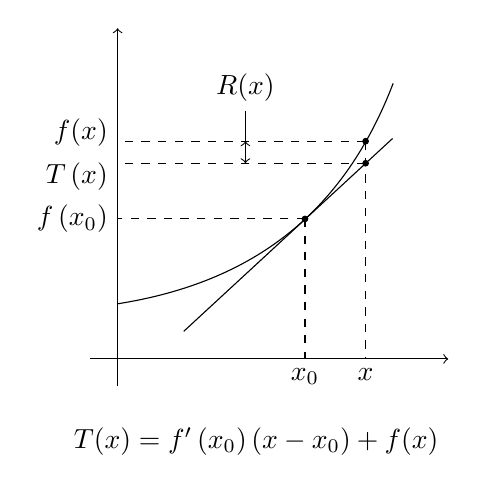
\begin{tikzpicture}[scale=0.7]
\draw[->](-0.5,0) -- (6,0);
\draw[->](0,-0.5) -- (0,6);
\draw [in=-111, out=9] (0,1) to (5,5);
\draw[fill=black] (3.4,2.54) circle (0.05);
\draw[dashed] (3.4,2.54) -- (3.4,0) node[anchor=north] {$x_0$};
\draw[dashed] (3.4,2.54) -- (0,2.54) node[anchor=east] {$f\left(x_0\right)$};

\draw[fill=black] (4.5,3.95) circle (0.05);
\draw[fill=black] (4.5,3.55) circle (0.05);
\draw[dashed] (3.4,2.54) -- (0,2.54);
\draw (0,3.3) node [anchor=east] {$T\left(x\right)$};
\draw (0,4.10) node[anchor=east] {$f(x)$};
\draw[dashed] (4.5,3.55) -- (0,3.55);

\draw[->] (2.32,4.5) -- (2.32,3.55);
\draw[->] (2.32,3.55) -- (2.32,3.95);
\draw (2.32,4.5) node[anchor=south] {$R(x)$};

\draw[dashed] (4.5,3.95) -- (4.5,0) node[anchor=north] {$x$};

\draw[dashed] (4.5,3.95) -- (0,3.95);
\draw  (1.2,0.5) to (4.99,4);

\draw (6,-1.5) node [anchor=east] {$T(x)=f'\left(x_0\right)\left(x-x_0\right)+f(x)$};

\end{tikzpicture}
\end{center}

\subsubsection*{Beispiel 5.4}
\begin{enumerate}
\item \begin{align*}
f:\R&\to\R\\
x&\to mx+b
\end{align*}
ist überall differenzierbar mit $f'\left( x\right)=m$, $\forall x\in\R$
\begin{align*}
f\left( x \right) - f\left( {{x_0}} \right)&= m\left( {x - {x_0}} \right)\\
\lim_{x \to {x_0}} \frac{{f\left( x \right) - f\left( {{x_0}} \right)}}{{\left( {x - {x_0}} \right)}}&= m
\end{align*}
\item $f\left( x\right)=\abs{x}$ ist für alle $x_0\not=0$ differenzierbar, aber nicht für $x_0=0$
\[f\left( x \right) - f\left( 0 \right) = \left\{ {\begin{array}{*{20}{c}}
x&{{\text{ für }}x \ge 0}\\
{ - x}&{{\text{ für }}x \le 0}
\end{array}} \right.\]
Also ist \[\frac{{f\left( x \right) - f\left( 0 \right)}}{{x - 0}} = \left\{ {\begin{array}{*{20}{c}}
1&{{\text{ fur }}x > 0}\\
{ - 1}&{{\text{ fur }}x < 0}
\end{array}} \right.\]
und besitzt also keinen Grenzwert für $x\to 0$, $x\not=0$
\item $\exp :\R\to\R$ ist überall auf $\R$ differenzierbar und $\exp'(x)=\exp(x)$. Sei $x_0\in\R$, $x_0\not=x=x_0+h\in\R$
\begin{align*}
\exp \left( {{x_0} + h} \right) - \exp \left( {{x_0}} \right)&= \exp \left( {{x_0}} \right)\left( {\exp \left( h \right) - 1} \right)\\
\exp \left( h \right) - 1&= h + \frac{{{h^2}}}{{2!}} +  \ldots \\
 \Rightarrow \frac{{\exp \left( h \right) - 1}}{h}&= 1 + \frac{h}{{2!}} + \frac{{{h^2}}}{{3!}}+\dots
\end{align*}
Also
\begin{align*}
\abs{\frac{\exp \left(h\right) - 1}{h} - 1} &\le \abs{h} \left[ \frac{1}{2!} + \frac{\abs{h}}{3!} + \frac{\abs{h}^2}{4!} + \ldots \right] \\
&\le \abs{h}\left[ {1 + \abs{h} + \frac{\abs{h}^2}{2!} + \ldots} \right] \\
&\le \abs{h}\exp \left(h\right)
\end{align*}
Woraus
\[\lim_{\substack{h \to 0 \\ h\not  = 0}}{\frac{\exp \left( h \right) - 1}{h}} = 1\]
und somit
\begin{align*}
\exp' \left( {x_0} \right) &= \lim_{\substack{h \to 0 \\ h \not  = 0}}{\frac{\exp \left( {{x_0} + h} \right) - \exp \left( {x_0} \right)}{h}} \\
&= \lim_{h \to 0}{\exp \left( {x_0}\right)} \left( {\frac{\exp \left( h \right) - 1}{h}} \right) \\
&= \exp \left( {x_0} \right)
\end{align*}
folgt
\item $\sin(x)$ und $\cos(x)$ sind überall differenzierbar und
\begin{align*}
\sin'&=\cos\\
\cos'&=-\sin
\end{align*}
Mit den Additionsgesetzen:
\begin{align*}
\sin \left( {x + h} \right) - \sin \left( x \right) &= \sin \left( x \right)\cos \left( h \right) + \cos \left( x \right)\sin \left( h \right) - \sin \left( x \right)\\
& = \sin \left( x \right)\left( {\cos \left( h \right) - 1} \right) + \cos \left( x \right)\sin \left( h \right)
\end{align*}
Nun ist
\[\mathop {\lim }\limits_{h \to 0} \frac{{\sin \left( h \right)}}{h} = 1\]
und
\begin{align*}
\frac{{\cos \left( h \right) - 1}}{h} &= \frac{{{{\cos }^2}\left( h \right) - 1}}{{h\left( {\cos \left( h \right) + 1} \right)}} = \frac{{{{\sin }^2}\left( h \right)}}{{h\left( {\cos \left( h \right) + 1} \right)}}\\
& = \frac{1}{{\mathop {\cos \left( h \right) + 1}\limits_{\begin{array}{*{20}{c}}
 \downarrow \\
{\frac{1}{2}}
\end{array}} }} \cdot \frac{{{{\sin }^2}\left( h \right)}}{{\mathop h\limits_{\begin{array}{*{20}{c}}
 \downarrow \\
0
\end{array}} }}
\end{align*}
\todo[inline]{There is a sin h/h which doesn't seem to belong anywhere, page 188 bottom right corner}
\begin{align*}
\frac{{\sin \left( {x + h} \right) - \sin \left( x \right)}}{h} &= \sin \left( x \right)\left( {\frac{{\cos \left( h \right) - 1}}{h}} \right) + \cos \left( x \right)\frac{{\sin \left( h \right)}}{h}\\
 \Rightarrow \mathop {\lim }\limits_{h \to 0} \frac{{\sin \left( {x + h} \right) - \sin \left( x \right)}}{h} &= \lim \left( {\sin \left( x \right)\mathop {\lim }\limits_{h \to 0} \left( {\frac{{\cos \left( h \right) - 1}}{h}} \right)} \right.\\
&\left. { \hspace{3mm}+ \cos \left( x \right)\mathop {\lim }\limits_{h \to 0} \left( {\frac{{\sin \left( h \right)}}{h}} \right)} \right)\\
 &= \sin \left( x \right)\lim \left( {\frac{{\cos \left( h \right) - 1}}{h}} \right)\\
 &\hspace{3mm}+ \cos \left( x \right)\lim \left( {\frac{{\sin \left( h \right)}}{h}} \right)\\
& = \left( {\sin \left( x \right)} \right) \cdot 0 + \left( {\cos \left( x \right)} \right) \cdot 1 = \cos \left( x \right)
\end{align*}
Analog
\begin{align*}
\cos \left( {x + h} \right) - \cos \left( x \right) &= \cos \left( x \right)\cos \left( h \right) - \sin \left( x \right)\sin \left( h \right) - \cos \left( x \right)\\
& = \cos \left( x \right)\left( {\cos \left( h \right) - 1} \right) + \sin \left( x \right)\sin \left( h \right)
\end{align*}
Da wie oben $\frac{{\cos \left( h \right) - 1}}{h} \to 0$, $\frac{{\sin \left( h \right)}}{{\left( h \right)}} \to 1$, folgt $\cos'=-\sin$
\end{enumerate}
Der Zusammenhang zwischen Differenzierbarkeit und Sstetigkeit ist:
\subsubsection*{Satz 5.5}\label{satz5.5}
Sei $\Omega\subseteq\R$, $x_0\in\Omega$ und $f:\Omega\to\R$ in $x_0$ differenzierbar. Dann ist $f$ in $x_0$ stetig. (Also ist ``Differenzierbarkeit'' ist mehr als ``Stetigkeit'')
\begin{beweis}{}
$f$ differenzierbar in $x_0$. Sei
\begin{align*}
T:\Omega \setminus \left\{ {x_0} \right\} & \to\R \\
x & \mapsto \frac{f\left( x \right) - f\left( {{x_0}} \right)}{x - {x_0}}
\end{align*}

Da $f$ differenzierbar in $x_0$ ist, hat $T$ ein Grenzwert in $x_0$, und
\[\mathop {\lim }\limits_{x \to {x_0}} T\left( x \right) = f'\left( x \right)\]
Für $x\not=x_0$
\[f\left( x \right) = T\left( x \right)\left( {x - {x_0}} \right) + f\left( {{x_0}} \right)\]
$f\left( x \right)$ ist die Summe von zwei Funktionen $T\left( x\right)\left( x-x_0\right)$ und $f\left( x_0\right)=$ konstant.\\

Da beide Funktionen einen Grenzwert an der Stelle $x_0$ besitzen, hat auch $f$ einen Grenzwert in $x_0$ und
\begin{align*}
\mathop {\lim }\limits_{x \to {x_0}} f\left( x \right)&= \mathop {\lim }\limits_{x \to {x_0}} \left( {T\left( x \right)} \right)\mathop {\lim }\limits_{x \to {x_0}} \left( {x - {x_0}} \right) + \mathop {\lim }\limits_{x \to {x_0}} f\left( {{x_0}} \right)\\
&= f'\left( x \right) \cdot 0 + f\left( {{x_0}} \right)= f\left( {{x_0}} \right)
\end{align*}
$\Rightarrow$ ist stetig in $x_0$.
\end{beweis}
\subsubsection*{Bemerkung}
Die Umkehrung von Satz 5.5 (s.~\pageref{satz5.5}) gilt nicht, z.B. $f\left( x \right)=\abs{x}$ ist stetig in $x=0$ aber nicht differenzierbar.

\subsubsection*{Beispiel 5.6}
Das folgende Beispiel zeigt, dass es stetige Funktionen $f:\R\to\R$ gibt, die an keiner Stelle $x_0\in\R$ differenzierbar sind. (Von der Waerden (1930))\\

\noindent Sei für $x\in\R$
\begin{align*}
<x> &=\text{Distanz von $x$ zur nächsten ganzen Zahl}\\
&=\min\left\{ \abs{ x-m}:m\in\mathbb{Z}\right\}
\end{align*}
Der Graph von $<x>$ sieht so aus
\begin{center}
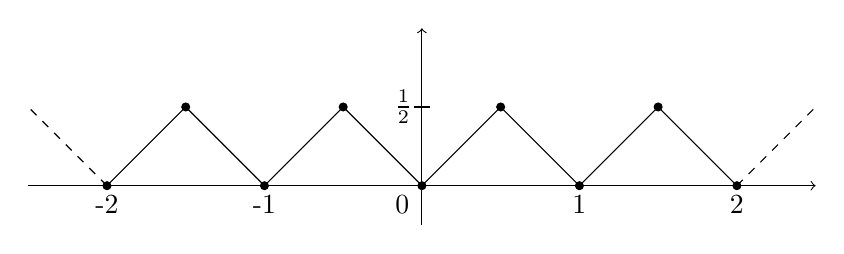
\begin{tikzpicture}[]
\draw[->](-5,0) -- (5,0);
\draw[->](0,-0.5) -- (0,2);

\draw (-4,0) node [anchor=north] {-2};
\draw (-2,0) node [anchor=north] {-1};
\draw (-0.25,0) node [anchor=north] {0};
\draw (2,0) node [anchor=north] {1};
\draw (4,0) node [anchor=north] {2};
\draw (0,1) node [anchor=east] {$1\over 2$};
\draw (-0.1,1) -- (0.1,1);


\draw (-4,0) -- (-3,1)--(-2,0) -- (-1,1)--(0,0)-- (1,1)-- (2,0)-- (3,1)-- (4,0);
\draw[fill=black] (-4,0) circle (0.05);
\draw[fill=black] (-3,1) circle (0.05);
\draw[fill=black] (-2,0) circle (0.05);
\draw[fill=black] (-1,1) circle (0.05);
\draw[fill=black] (0,0) circle (0.05);
\draw[fill=black] (1,1) circle (0.05);
\draw[fill=black] (2,0) circle (0.05);
\draw[fill=black] (3,1) circle (0.05);
\draw[fill=black] (4,0) circle (0.05);
\draw[dashed] (4,0)--(5,1);
 \draw[dashed] (-4,0)--(-5,1);
\end{tikzpicture}
\end{center}
Graph von $\frac{10x}{10}$
\begin{center}
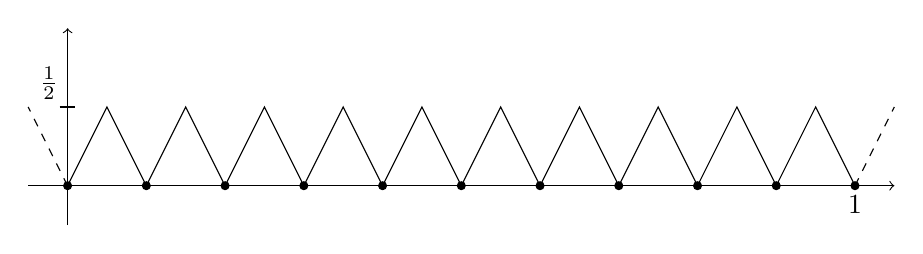
\begin{tikzpicture}[]
\draw[->](-0.5,0) -- (10.5,0);
\draw[->](0,-0.5) -- (0,2);


\draw (10,0) node [anchor=north] {1};

\draw[fill=black] (10,0) circle (0.05);
\draw[fill=black] (9,0) circle (0.05);
\draw[fill=black] (8,0) circle (0.05);
\draw[fill=black] (7,0) circle (0.05);
\draw[fill=black] (6,0) circle (0.05);
\draw[fill=black] (5,0) circle (0.05);
\draw[fill=black] (4,0) circle (0.05);
\draw[fill=black] (3,0) circle (0.05);
\draw[fill=black] (2,0) circle (0.05);
\draw[fill=black] (1,0) circle (0.05);
\draw[fill=black] (0,0) circle (0.05);

\draw (0,1.3) node [anchor=east] {$1\over 2$};
\draw (-0.1,1) -- (0.1,1);


\draw (0,0)--(0.5,1)-- (1,0)--(1.5,1)--(2,0)--(2.5,1)--(3,0)--(3.5,1)--(4,0)--(4.5,1)--(5,0)--(5.5,1)-- (6,0)--(6.5,1)--(7,0)--(7.5,1)--(8,0)--(8.5,1)--(9,0)--(9.5,1)--(10,0);
\draw[dashed] (10,0) -- (10.5,1);
\draw[dashed] (0,0) -- (-0.5,1);


\end{tikzpicture}
\end{center}
Sei
\[f\left( x \right): =  < x >  + \frac{{ < 10x > }}{{10}} + \frac{{ < {{10}^2}x > }}{{100}} +  \ldots \]
Da
\[0 \le  < {10^n}x >  \le \frac{1}{2}\]
folgt absolute Konvergenz. Ausserdem sei
\[{f_k}\left( x \right) = \sum\limits_{n = 0}^k {\frac{{ < {{10}^n}x > }}{{{{10}^n}}}} \]
Dann ist
\[\abs{ {f\left( x \right) - {f_k}\left( x \right)} } = \abs{ {\sum\limits_{n = k + 1}^\infty  {\frac{{ < {{10}^n}x > }}{{{{10}^n}}}} } } \le \frac{1}{2}\abs{ {\sum\limits_{n = k + 1}^\infty  {\frac{1}{{{{10}^n}}}} } } = \frac{1}{2} \cdot \frac{{{{10}^{ - k}}}}{9}\]
$\forall k\geq 1$ ist $f_k:\R\to\R$ stetig. \\

Da die Folge $\left( f_k\right)_{k\geq 1}$ gleichmässig gegen $f$ konvergiert, ist $f$ stetig. Man kann zeigen, dass $f$ in keinem Punkt von $\R$ differenzierbar ist. \todo{End of beweis is put here, I think it is better if it stays up when the bsp begins. Page 192 middle}
\subsubsection*{Satz 5.7}
Seien $f,g:\Omega\to\R$ Funktionen, $x_0\in\R$. Wir nehmen an, dass $f$ und $g$ in $x_0$ differenzierbar sind. Dann sind $f+g$, $f\cdot g$ und falls $g\left( x_0\right)\not=0$ auch $f/g$\todo{Is this supposed to be a fraction?? page 192 bottom; limenet: yes, function f over function g} an der Stelle $x_0$ differenzierbar. Es gelten dann folgende Formeln:
\begin{enumerate}
\item $\left( {af + bg} \right)'\left( {{x_0}} \right) = af'\left( {{x_0}} \right) + bf'\left( {{x_0}} \right)\hspace{5mm}\forall a,b \in \R$
\item \label{satz5.7,2.}$\left( {f \cdot g} \right)'\left( {{x_0}} \right) = f'\left( {{x_0}} \right) \cdot g\left( {{x_0}} \right) + f\left( {{x_0}} \right) \cdot g'\left( {{x_0}} \right)$
\item $\left( {\frac{f}{g}} \right)'\left( {{x_0}} \right) = \frac{{f'\left( {{x_0}} \right) \cdot g\left( {{x_0}} \right) - f\left( {{x_0}} \right) \cdot g'\left( {{x_0}} \right)}}{{g{{\left( {{x_0}} \right)}^2}}}$
\end{enumerate}
\begin{beweis}{}
\begin{enumerate}
\item Für $x\not=x_0$
\[\frac{{\left( {af + bg} \right)\left( x \right) - \left( {af + bg} \right)\left( {{x_0}} \right)}}{{x - {x_0}}} = a\left( {\frac{{f\left( x \right) - f\left( {{x_0}} \right)}}{{x - {x_0}}}} \right) + b\left( {\frac{{g\left( x \right) - g\left( {{x_0}} \right)}}{{x - {x_0}}}} \right)\]
Da $f$ und $g$ in $x_0$ differenzierbar sind, folgt, dass $af+bg$ in $x_0$ differenzierbar ist und
\[\left( {af + bg} \right)\left( {{x_0}} \right) = af'\left( {{x_0}} \right) + bf'\left( {{x_0}} \right)\]
\item \[f\left( x \right)g\left( x \right) - f\left( {{x_0}} \right)g\left( {{x_0}} \right) = g\left( x \right)\left[ {f\left( x \right) - f\left( {{x_0}} \right)} \right] + f\left( {{x_0}} \right)\left[ {g\left( x \right) - g\left( {{x_0}} \right)} \right]\]
Durch $\left( x-x_0\right)$ dividiert
\begin{align*}
\frac{{f\left( x \right)g\left( x \right) - f\left( {{x_0}} \right)g\left( {{x_0}} \right)}}{{x - {x_0}}} &= \frac{{f\left( x \right) - f\left( {{x_0}} \right)}}{{\left( {x - {x_0}} \right)}} \cdot g\left( {{x_0}} \right)\\
 &+ \frac{{g\left( x \right) - g\left( {{x_0}} \right)}}{{\left( {x - {x_0}} \right)}} \cdot f\left( {{x_0}} \right)
\end{align*}
Da $g$ in $x_0$ differenzierbar ist, ist $g$ in $x_0$ stetig und (Satz 5.5, s.~\pageref{satz5.5})
\[\mathop {\lim }\limits_{x \to {x_0}} g\left( x \right) = g\left( {{x_0}} \right)\]
Die Formel folgt dann aus der Differenzierbarkeit von $f$ und $g$ in $x_0$
\item \begin{align*}
\frac{{f\left( x \right)}}{{g\left( x \right)}} - \frac{{f\left( {{x_0}} \right)}}{{g\left( {{x_0}} \right)}} &= \frac{{f\left( x \right)g\left( {{x_0}} \right) - f\left( {{x_0}} \right)g\left( x \right)}}{{g\left( x \right)g\left( {{x_0}} \right)}}\\
 &= \frac{{\left[ {f\left( x \right) - f\left( {{x_0}} \right)} \right]g\left( {{x_0}} \right) - f\left( {{x_0}} \right)\left[ {g\left( x \right) - g\left( {{x_0}} \right)} \right]}}{{g\left( x \right)g\left( {{x_0}} \right)}}
\end{align*}
Man dividiere duch $x-x_0$ und benutze die Stetigkeit von $g$ in $x_0$
\end{enumerate}
\end{beweis}
\subsubsection*{Beispiel 5.8}
\begin{enumerate}
\item $n\in\N$, $f_n\left( x\right)=x^n$ ist überall differenzierbar und $f'_n\left( x\right) = nx^{n-1}$
\begin{beweis}{}
Induktion: $f_0\left( x\right) = 1$ $\forall x$ \[f'_0\left( x\right) = 0 \left( = 0\cdot x^{-1}\right)\]
\begin{itemize}
\item $f_1\left( x\right) = x$, $\forall x$
\item $f'_1\left( x\right) = 1 = 1\cdot x^{1-1}$ $\checkmark$
\end{itemize}
Sei $n\geq 2$. Wir nehmen an, dass die Formel für $n-1$ gilt, i.e.
\begin{align*}
f{'_{n - 1}}\left( x \right) &= \left( {{x^{n - 1}}} \right)' = \left( {n - 1} \right){x^{n - 2}}\\
{f_n}\left( x \right) &=  {x^n} = x \cdot {x^{n - 1}} = x \cdot {f_{n - 1}}\left( x \right)
\end{align*}
Nach 2., Satz 5.7 (s.~\pageref{satz5.7,2.})
\begin{align*}
f{'_n}\left( x \right) &= \left( x \right)'{f_{n - 1}}\left( x \right) + xf{'_{n - 1}}\left( x \right)\\
 &= {f_{n - 1}}\left( x \right) + x\left( {n - 1} \right){x^{n - 2}}\\
 &= {x^{n - 1}} + \left( {n - 1} \right){x^{n - 1}} = n{x^{n - 1}}
\end{align*}
\end{beweis}
\item \begin{align*}
p(x)&=a_nx^n+a_{n-1}x^{n-1}+\dots+a_0\\
p'(x)&=na_nx^{n-1}+\left( n-1\right)a_{n-1}x^{n-2}+\dots+a_1
\end{align*}
Insbesondere ist die Ableitung eines Polynoms von Grad $n$ ein Polynom von Grad $\left( n-1\right)$, $n\geq 1$.
\item Sei $R(x)=\frac{p(x)}{q(x)}$, wobei $p,q$ Polynome bezeichnen. $R(x)$ ist eine sogenannte rationale Funktion mit Definitionsbereich
\[\Omega = \left\{ x\in\R : q(x)\not=0\right\}\]
\[R'(x) = \frac{{p'(x)q(x) - p(x)q'(x)}}{{{q^2}(x)}}\]
z.B. \[R(x) = \frac{{{x^3} + 1}}{{x - 1}}\]
\begin{align*}
R(x) &= \frac{{\left( {3{x^2}} \right)\left( {x - 1} \right) - \left( {{x^3} + 1} \right)}}{{{{\left( {x - 1} \right)}^2}}}\\
 &= \frac{{3{x^3} - 3{x^2} - {x^3} - 1}}{{{{\left( {x - 1} \right)}^2}}}\\
 &= \frac{{2{x^3} - 3{x^2} - 1}}{{{{\left( {x - 1} \right)}^2}}}
\end{align*}
\end{enumerate}
Die nächste Rechenregel wird uns erlauben, Funktionen wie z.B. $\exp\left( x^3+1\right)$ und $\sin\left( x^2\right)$ abzuleiten

\subsubsection*{Satz 5.9 (Kettenregel)}
Seien $f:\Omega\to\R$, $g:T\to\R$ Funktionen mit $f\left( \Omega\right)\subset T$, und $x_0\in\Omega$. Wir nehmen an, dass $f$ an der Stelle $x_0$ und $g$ an der Stelle $f\left( x_0\right)$, differenzierbar sind. Dann ist $g\circ f:\Omega\to\R$ an der Stelle $x_0$ differenzierbar und
\[\left( {g\circ f} \right)'\left( {{x_0}} \right) = g'\left( {f\left( {{x_0}} \right)} \right)f'\left( {{x_0}} \right)\]

\subsubsection*{Bemerkung}
$f$ ist differenzierbar in $x_0$, falls
\[\mathop {\lim }\limits_{\begin{array}{*{20}{c}}
{x \to {x_0}}\\
{x\not  = {x_0}}
\end{array}} \frac{{f\left( x \right) - f\left( {{x_0}} \right)}}{{x - {x_0}}}\]
existiert, d.h. für jede in $\Omega\backslash\{ x_0\}$ enthaltene Folge $\left( x_n\right)_{n\geq 1}$ mit Grenzwert $x_0$, existiert der Limes
\[\mathop {\lim }\limits_{n \to \infty } \frac{{f\left( {{x_n}} \right) - f\left( {{x_0}} \right)}}{{{x_n} - {x_0}}}\]

\begin{beweis}{}
Sei $\left( x_n\right)_{n\geq 1}$ mit $\lim x_n=x_0$, $x_n\not=x_0$. Dann gilt
\[\lim f\left( x_n\right) = f\left( x_0\right)\]
(Nach Satz 5.5, s.~\pageref{satz5.5},  $f$ differenzierbar $\Rightarrow$ $f$ stetig (in $x_0$)).\\

\noindent Sei $y_n:=f\left( x_n\right)$ $\left( y_0:=f\left( x_0\right)\right)$. Wir nehmen an, dass $y_n\not=f\left( x_0\right)$, $\forall n$. Dann folgt
\begin{align*}
\frac{{\left( {g \circ f} \right)\left( {{x_n}} \right) - \left( {g \circ f} \right)\left( {{x_0}} \right)}}{{{x_n} - {x_0}}} &= \frac{{g\left( {f\left( {{x_n}} \right)} \right) - g\left( {f\left( {{x_0}} \right)} \right)}}{{x - {x_0}}}\\
&= \left( {\frac{{g\left( {f\left( {{x_n}} \right)} \right) - g\left( {f\left( {{x_0}} \right)} \right)}}{{f\left( {{x_n}} \right) - f\left( {{x_0}} \right)}}} \right) \cdot \left( {\frac{{f\left( {{x_n}} \right) - f\left( {{x_0}} \right)}}{{x - {x_0}}}} \right)\\
& = \mathop {\left( {\frac{{g\left( {{y_n}} \right) - g\left( {{x_0}} \right)}}{{{y_n} - {y_0}}}} \right)}\limits_{\begin{array}{*{20}{c}}
{\begin{array}{*{20}{c}}
 \downarrow &{\mathop {\lim }\limits_{n \to \infty } }
\end{array}}\\
{\begin{array}{*{20}{c}}
{g'\left( {{y_0}} \right)}&{{\text{         }}}
\end{array}}
\end{array}}  \cdot \mathop {\left( {\frac{{f\left( {{x_n}} \right) - f\left( {{x_0}} \right)}}{{x - {x_0}}}} \right)}\limits_{\begin{array}{*{20}{c}}
{\begin{array}{*{20}{c}}
 \downarrow &{\mathop {\lim }\limits_{n \to \infty } }
\end{array}}\\
{\begin{array}{*{20}{c}}
{f'\left( {{x_0}} \right)}&{{\text{         }}}
\end{array}}
\end{array}} \\
&\hspace{-1.5mm}\mathop  = \limits^{n \to \infty } g'\left( {f\left( {{x_0}} \right)} \right)f'\left( {{x_0}} \right)
\end{align*}
\end{beweis}
\subsubsection*{Beispiel 5.10}
\begin{enumerate}
\item Berechne die Ableitung von $\exp\left( x^3+1\right)$
\[\begin{array}{*{20}{l}}
{g\left( x \right) = \exp \left( x \right)}&{f\left( x \right) = {x^3} + 1}\\
{g'\left( x \right) = \exp \left( x \right)}&{f'\left( x \right) = 3{x^2}}
\end{array}\]
\begin{align*}
\left( g\circ f\right) \left( x\right) &= \exp\left( x^3+1\right)\\
\left( g\circ f\right)' \left( x\right) &= g'\left( f\left( x\right)\right)\cdot f'\left( x\right)=\left[ \exp\left( x^3+1\right) \right]\cdot 3x^2
\end{align*}
\item \[ \left( \sin\left( x^2\right) \right)'=\left( g\circ f\right)'\left( x\right)\] mit
\[\begin{array}{*{20}{l}}
{g\left( x \right) = \sin \left( x \right)}&{f\left( x \right) = {x^2}}\\
{g'\left( x \right) = \cos \left( x \right)}&{f'\left( x \right) = 2x}
\end{array}\]
\[\left( \sin\left( x^2\right) \right)'=\cos\left( x^2\right)\cdot 2x\]
\item \[\left( {{{\left( {3{x^7} + 11{x^6} + 5} \right)}^2}} \right)' = 2\left( {3{x^7} + 11{x^6} + 5} \right) \cdot \left( {21{x^6} + 66{x^5}} \right)\]
\item Sei $g:\R\to\R$ differenzierbar und $n\in\N$ \[ f\left( x\right) = g\left( x\right)^n\]
Dann ist \[f'\left( x\right)=ng\left( x\right)^{n-1}\cdot g'\left( x\right)\]
\item \begin{align*}
\exp\left( \exp\left( x\right)\right)&=e^{e^x}\\
\left( e^{e^x}\right)'&=e^{\left( e^x\right)}\cdot e^x
\end{align*}
\end{enumerate}

\section{Der Mittelwertsatz und Folgerungen}
Wichtige Informationen über eine Funktion $f$ lassen sich leicht aus der Ableitung schliessen. Dies geschieht mittels dem Mittelwertsatz . Ein Spezialfalls der Mittelwertsatz ist
\subsubsection*{Satz 5.12}\label{satz5.12}
Sei $f:\lbrack a,b\rbrack\to\R$ stetig und auf $\left( a,b\right)$ differenzierbar. Sei $z_+\in\lbrack a,b\rbrack$ mit $f\left( z_+\right) =\max\left\{ f\left( x\right) : x\in\lbrack a,b\rbrack\right\}$. Wir nehmen an, dass $z_+\in\left( a,b\right)$. Dann gilt $f'\left( z_+\right) = 0$ Eine analoge Aussage gilt für $z_{-}$.
\subsubsection*{Bemerkung 5.13}
\begin{enumerate}
\item $z_+$, $z_-$ existieren nach Satz 4.9
\item Die Voraussetzung $z_+\in\left( a,b \right)$ ist wichtig, z.B. Sei $f:\lbrack 0,1\rbrack\to\R$, $f(x)=x$. Dann ist $z_+=1$ und $f'(x)=1\not=0$ $\left( \forall x\in\left( a,b\right)\right)$
\end{enumerate}

\begin{beweis}{}
Sei $z_+\in\left( a,b\right)$. Da $\left( a,z_+\right)\not=\varnothing$ und $\left( z_+,b\right)\not=\varnothing$, gibt es
\[\left( x_n\right)_{n\geq 1}\subset\left( a,z_+\right)\]
sowie
\[\left( y_n\right)_{n\geq 1}\subset\left( z_+,b\right)\]
mit
\[\mathop {\lim }\limits_{n \to \infty } {x_n} = {z_ + } = \mathop {\lim }\limits_{n \to \infty } {y_n}\]
$\left( \text{z.B. }{x_n} = {z_ + } - \frac{1}{n}, {y_n} = {z_ + } + \frac{1}{n}\right)$\\

Für $n\geq 1$ folgt

\begin{align*}
f'\left( {{z_ + }} \right) &= \mathop {\lim }\limits_{n \to \infty } \frac{{\overbrace {f\left( {{x_n}} \right) - f\left( {{z_ + }} \right)}^{ < 0}}}{{\underbrace {{x_n} - {z_ + }}_{ < 0}}} \ge 0\\
f\left( {{z_ + }} \right) &= \max \left\{ {f\left( x \right)} \right\}\\
f'\left( {{z_ + }} \right) &= \mathop {\lim }\limits_{n \to \infty } \frac{{\overbrace {f\left( {{y_n}} \right) - f\left( {{z_ + }} \right)}^{ < 0}}}{{\underbrace {{y_n} - {z_ + }}_{ > 0}}} \le 0
\end{align*}
Woraus \[ f'\left( z_+\right) = 0\] folgt.
\end{beweis}

\subsubsection*{Satz 5.14 (Mittelwertsatz)}\label{satz5.14}
Sei $f:\lbrack a,b\rbrack\to\R$ stetig und auf $\left( a,b\right)$ differenzierbar, $a\not=b$. Dann gibt es $x_0\in\left( a,b\right)$ mit \[f'\left( {{x_0}} \right) = \frac{{f\left( b \right) - f\left( a \right)}}{{b - a}}\]
\begin{center}
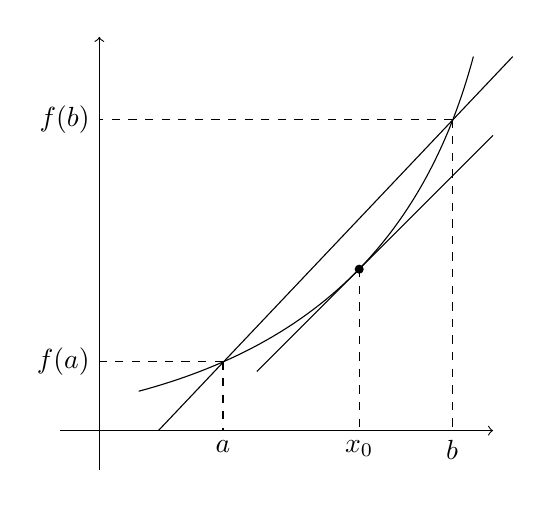
\begin{tikzpicture}
\node [] (0) at (5, 0) {};
\node [] (1) at (0, 5) {};
\node [] (2) at (0, -0.5) {};
\node [] (3) at (-0.5, 0) {};
\node [] (4) at (0.5, 0.5) {};
\node [] (5) at (4.75, 4.75) {};
\node [] (6) at (5, 3.75) {};
\node [] (7) at (2, 0.75) {};
\node [] (8) at (0.75, 0) {};
\node [] (9) at (5.25, 4.75) {};
\draw [->] (3.center) to (0.center);
\draw [->] (2.center) to (1.center);
\draw [bend right] (4.center) to (5.center);
\draw [] (7.center) to (6.center);
\draw [] (8.center) to (9.center);
\draw[dashed] (1.57,0.88) --  (0,0.88) node [anchor=east]{$f(a)$};
\draw[dashed] (1.57,0.88) -- (1.57,0) node [anchor=north]{$a$};
\draw[dashed] (4.48,3.95) -- (0,3.95) node [anchor=east]{$f(b)$};
\draw[dashed] (4.48,3.95)--(4.48,0) node [anchor=north]{$b$};
\draw[fill=black] (3.3,2.05) circle (0.05);
\draw[dashed] (3.3,2.05)--(3.3,0) node [anchor=north]{$x_0$};



\end{tikzpicture}
\end{center}

\begin{beweis}{}
Die Idee lässt sich auf den Fall $f(a)=f(b)=0$ züruckführen und dann den Satz 5.12 (s.~\pageref{satz5.12}) anwenden. Die Gleichung für die Sekante durch die Punkte $\left( a,f(a)\right)$, $\left( b,f\left( b\right)\right)$ ist
\[S\left( x \right) = \left( {x - a} \right)\left( {\frac{{f\left( b \right) - f(a)}}{{b - a}}} \right) + f\left( a \right)\]
Sei nun $g(x)=f(x)-S(x)$. Dann ist $g(a)=0=g(b)$\\

\noindent\underline{Fall 1:} $g$ ist identisch $=0$. Also ist $f(x)=S(x)$ eine Gerade und die Aussage stimmt $\forall x_0\in\left( a,b\right)$ \\

\noindent\underline{Fall 2:} $g\not=0$. Also ist entweder
\[\mathop {\max }\limits_x g(x) > 0\text{ }\left(\text{oder }\mathop {\min }\limits_x g(x) < 0\right)\]
Im ``$\max$''-Fall sei $z_+$ mit
\[g\left( {{z_ + }} \right) = \max \left\{ {g(x):x \in \left[ {a,b} \right]} \right\}\]
Dann ist $ {{z_ + }} \in\left( a,b\right)$ (Da $g(a)=g(b)=0$, und $g\left( {{z_ + }} \right) >0$) und nach Satz 5.12 (s.~\pageref{satz5.12}) $g'\left( z_+\right)=0$, d.h.
\begin{align*}
g\left( {{z_ + }} \right) &= f'\left( {{z_ + }} \right) - S'\left( {{z_ + }} \right) = 0\\
 \Rightarrow f'\left( {{z_ + }} \right) &= S'\left( {{z_ + }} \right) = \frac{{f\left( b \right) - f\left( a \right)}}{{b - a}}
\end{align*}
Der ``$\min$''-Fall ist analog.
\end{beweis}
Als erste Anwendung haben wir
\subsubsection*{Korollar 5.15}
Sei $f:\lbrack a,b\rbrack\to\R$ wie im Satz 5.14 (s.~\pageref{satz5.14})
\begin{enumerate}
\item Falls $f'(x)=0$, $\forall x\in\left( a,b\right)$ folgt, dass $f$ konstant ist.
\item Falls $f'(x)\geq 0$, $\forall x\in\left( a,b\right)$ so ist $f$ monoton wachsend.
\item Falls $f'(x)> 0$, $\forall x\in\left( a,b\right)$ so ist $f$ streng monoton wachsend.
\item Falls $f'(x)\leq 0$, $\forall x\in\left( a,b\right)$ so ist $f$ monoton fallend.
\item Falls $f'(x)< 0$, $\forall x\in\left( a,b\right)$ so ist $f$ streng monoton fallend.
\end{enumerate}

\begin{beweis}{}
\begin{enumerate}
\item Seien $a\leq x<y\leq b$ beliebig und sei (nach Mittelwertsatz) $x_0\in\left( x,y\right)$ mit
\[\frac{{f\left( y \right) - f\left( x \right)}}{{y - x}} = f'\left( {{x_0}} \right)\]
da $f'\left( x_0\right)$ folgt $f\left( y\right)=f(x)\Rightarrow f$ ist konstant
\item Seien $a\leq x<y\leq b$ beliebig und  $x_0\in\left( x,y\right)$ mit
\[\frac{{f\left( y \right) - f\left( x \right)}}{{y - x}} = f'\left( {{x_0}}>0 \right)\]
woraus folgt  $f\left( y\right)\geq f(x)$  folgt $\Rightarrow f$ monoton wachsend.
\item Analog
\item Analog
\end{enumerate}
\end{beweis}

\subsubsection*{Beispiel 5.16}
\begin{enumerate}
\item Bestimme alle differenzierbare Funktionen $f:\R\to\R$ mit $f'=\lambda f$. Offensichtlich erfüllt $t\to e^{\lambda t}$ diese Gleichung
\begin{align*}
f\left( t\right)&=e^{\lambda t}\\
f'\left( t\right)&=\lambda e^{\lambda t}=\lambda f\left( t\right)
\end{align*}
Betrachten wir
\begin{align*}
g\left( t\right)&=e^{-\lambda t}f\left( t\right)\\
g'\left( t \right) &=  - \lambda {e^{ - \lambda t}}f\left( t \right) + {e^{ - \lambda t}}f'\left( t \right)\\
 &= {e^{ - \lambda t}}\left( { - \lambda f\left( t \right) + f'\left( t \right)} \right)\\
 &= {e^{ - \lambda t}}\left( 0 \right)\forall t\\
 &= 0
\end{align*}
Also folgt, dass $g$ konstant ist, d.h.
\[g\left( t \right) = C \Rightarrow f\left( t \right) = C{e^{\lambda t}}\]
\underline{Anders gesagt:} Die Menge der Lösungen von $f'=\lambda f$ ist ein $1-$dimensionaler Vektorraum
\[V = \left\{ {f:\R \to\R \mid f' = \lambda f} \right\} = \left\{ {C{e^{\lambda t}}\mid c \in \R} \right\}\]
\item \begin{align*}
f\left( x \right) &= \frac{{2x}}{{1 + {x^2}}}\\
f'\left( x \right) &= \frac{{2\left( {1 + {x^2}} \right) - \left( {2x} \right)\left( {2x} \right)}}{{{{\left( {1 + {x^2}} \right)}^2}}}\\
 &= \frac{{2 - 2{x^2}}}{{{{\left( {1 + {x^2}} \right)}^2}}} = \frac{{2\left( {1 - {x^2}} \right)}}{{{{\left( {1 + {x^2}} \right)}^2}}}
\end{align*}
\begin{align*}
&f'\left( x \right) < 0\text{ für }\abs{x}>1\\
&f'\left( { \pm 1} \right) = 0\\
&f'\left( x \right) > 0\text{ für }\abs{x}<1
\end{align*}
%THIS IS A PRETTY AWFUL WAY OF CENTERING THE ROWS, BUT IT WORKS :)
\begin{tabularx}{\textwidth}{|Y|Y|Y|Y|Y|}
\hline
    $x$ & $x<-1$                          & $-1<x<0$ & $0<x<1$ & $x>1$                                                      \\\hline\hline
    \vspace{-1mm}$f'\left( x\right)$        & \vspace{-1mm}$-$ & \vspace{-1mm}$+$ & \vspace{-1mm}$+$ & \vspace{-1mm}$-$ \\ [1.5ex]\hline
    \vspace{-1mm}$f\left( x\right)$                  & \vspace{-1mm}$\searrow$     & \vspace{-1mm}$\nearrow$ & \vspace{-1mm}$\nearrow$ & \vspace{-1mm}$\searrow$                  \\[1.5ex]\hline
 \end{tabularx}

\begin{center}
\begin{tikzpicture}[scale=0.5]
\node [] (0) at (-3, -2) {};
\node [] (1) at (3, 2) {};
\node [] (2) at (10, 0.5) {};
\node [] (3) at (-10, -0.5) {};
\draw [, in=-165, out=15, looseness=1.25] (0.center) to (1.center);
\draw [, in=180, out=15, looseness=0.75] (1.center) to (2.center);
\draw [, in=-15, out=-165] (0.center) to (3.center);
\draw[->] (0,-4) -- (0,4);
\draw[<-] (10,0) -- (-10,0);
\draw[fill=black] (0,0) circle (0.125);
\draw[fill=black] (3.75,2.1) circle (0.125);
\draw[fill=black] (3.75,0.2) --(3.75,-0.2) node[anchor=north] {1};


\draw[fill=black] (-4,-2.2) circle (0.125);
\draw[fill=black] (-4,0.2) --(-4,-0.2) node[anchor=north] {$-1$};
\end{tikzpicture}
\end{center}

\end{enumerate}

\subsubsection*{Korollar 5.17 (Bernoulli, L'Hôpital)}
Seien $f,g:\lbrack a,b\rbrack\to\R$ stetig differenzierbar in $\left( a,b\right)$ mit $g'(x)\not=0$, $\forall x\in\left( a,b\right)$. Wir nehmen an, dass
\begin{enumerate}[(i)]
\item $f(a)=0=g(a)$
\item $\mathop {\lim }\limits_{x \searrow a} \frac{{f'\left( x \right)}}{{g'\left( x \right)}} = A$
\end{enumerate}
Dann ist $g(x)\not=0$, $\forall x>a$ und $\mathop {\lim }\limits_{x \searrow a} \frac{{f\left( x \right)}}{{g\left( x \right)}} = A$

\begin{beweis}{}
Falls es $x_1>a$ gibt mit $g\left( x_1\right)=0$, dann folgt die Existenz von $x_0\in\left( a,x_1\right)$ mit $g'\left( x_0\right)=0$ (MWS.)

\begin{center}
\begin{tikzpicture}
\draw (-3.5,0) --(3.5,0);
\draw[fill=black] (3,0) circle (0.05) node [anchor=north]{$x_1$};
\draw[fill=black] (-3,0) circle (0.05) node [anchor=north]{$a$};
\draw[bend left=60] (-3,0) to (3,0);
\draw[dashed] (0,0) -- (0,1.52);
\draw[fill=black] (0,1.52) circle (0.05);
\draw[] (-3,0) -- (-3,2.5);
\draw[] (3,0) -- (3,2.5);
\draw[] (-2,1.52) -- (2,1.52);
\end{tikzpicture}
\end{center}

Wiederspruch zur Annahme $g'(x)\not=0$, $\forall x\in\left( a,b\right)$. Also $g(x)\not=0$, $\forall x>a$. Nun sei $a<s<b$ beliebig, und
\[h\left( x \right): = \frac{{f\left( s \right)}}{{g\left( s \right)}} \cdot g\left( x \right) - f\left( x \right)\hspace{5mm}x \in \left[ {a,s} \right]\]
Dann gilt, $h(a)=0$ und $h(s)=0$, es gibt also $x_s\in\left( a,s\right)$ mit $h'\left( x_s\right)=0$, d.h.
\begin{align*}
0 &= h'\left( {{x_s}} \right) = \frac{{f\left( s \right)}}{{g\left( s \right)}} \cdot g'\left( {{x_s}} \right) - f'\left( {{x_s}} \right)\\
 \Rightarrow& \frac{{f'\left( {{x_s}} \right)}}{{g'\left( {{x_s}} \right)}} = \frac{{f\left( s \right)}}{{g\left( s \right)}}\tag{\textasteriskcentered}
\end{align*}
Sei nun $s_n\in\left( a,b\right)$ beliebig mit $\lim s_n=a$. Da $a<x_{s_n}<s_n$ folgt, $\lim x_{s_n}=a$, und aus (\textasteriskcentered)
\[\lim \frac{{f\left( {{s_n}} \right)}}{{g\left( {{s_n}} \right)}} = \lim \frac{{f'\left( {{x_{{s_n}}}} \right)}}{{g'\left( {{x_{{s_n}}}} \right)}} = A\]
\end{beweis}

\subsubsection*{Bemerkung 5.18}
\begin{enumerate}
\item Es gibt die selbe Version für $\mathop {\lim }\limits_{x \nearrow b} $
\item (Limes von links und rechts zusammen). Seien $f,g:\lbrack a,b\rbrack\to\R$ stetig. Sei $a<c<b$, wir nehmen an, $f,g$ sind in $\left( {a,c} \right) \cup \left( {c,b} \right)$ differenzierbar, $g'(x)\not=0$, $\forall x\in\left( {a,c} \right) \cup \left( {c,b} \right)$ und
\begin{enumerate}[(i)]
\item $f(c)=g(c)=0$
\item $\mathop {\lim }\limits_{\begin{array}{*{20}{c}}
{x \to c}\\
{x\not  = c}
\end{array}} \frac{{f'\left( x \right)}}{{g'\left( x \right)}} = A$
\end{enumerate}
Dann ist $g(x)\not=0$, $\forall x\in\left( {a,c} \right) \cup \left( {c,b} \right)$ und $\mathop {\lim }\limits_{\begin{array}{*{20}{c}}
{x \to c}\\
{x\not  = c}
\end{array}} \frac{{f\left( x \right)}}{{g\left( x \right)}} = A$
\end{enumerate}

\subsubsection*{Beispiel 5.19}
\begin{enumerate}
\item $\mathop {\lim }\limits_{x \to 1} \frac{{{x^3} - 1}}{{{x^2} - 1}} = \lim \frac{{3{x^2}}}{{2x}} = \frac{3}{2}$
\item $\mathop {\lim }\limits_{x \to 0} \frac{{\sin \left( x \right)}}{x} = \lim \frac{{\cos \left( x \right)}}{1} = 1$
\item $\mathop {\lim }\limits_{x \to 0} \frac{{\sin \left( {{x^2}} \right)}}{{{x^2}}} = \mathop {\lim }\limits_{x \to 0} \frac{{2x\cos \left( {{x^2}} \right)}}{{2x}} = \mathop {\lim }\limits_{x \to 0} \cos \left( {{x^2}} \right) = 1$
\item $\mathop {\lim }\limits_{x \to 0} \frac{{\cos \left( x \right) - 1}}{{{x^2}}} = \lim \frac{{ - \sin \left( x \right)}}{{2x}} =  - \frac{1}{2}$
\item $\mathop {\lim }\limits_{x \to 0} \frac{{\left( {{e^x} - 1 - x - \frac{{{x^2}}}{{2!}}} \right)}}{{{x^3}}} = \mathop {\lim }\limits_{x \to 0} \left( {\frac{{{e^x} - 1 - x}}{{3{x^2}}}} \right) = \mathop {\lim }\limits_{x \to 0} \frac{{{e^x} - 1}}{{6x}} = \mathop {\lim }\limits_{x \to 0} \frac{{{e^x}}}{6} = \frac{1}{6}$
\end{enumerate}
Die nächste Anwendung des Mittelwertsatzes ist der sogenannte ``Umkehrsatz''
\subsubsection*{Fundamentale Frage}
Sei $f:\R\to\R$ differenzierbar und bijektiv und sei $g:\R\to\R$ die inverse Funktion. Ist dann $g$ auch differenzierbar?

\subsubsection*{Beispiel}
\begin{align*}
f:\R&\to\R\\
x&\to x^3
\end{align*}
ist überall differenzierbar und bijektiv. Die ``Umkehrfunktion''
\begin{align*}
g:\R&\to\R\\
x&\to x^{1\over 3}
\end{align*}
ist aber in $0$ nicht differenzierbar
\[\frac{{g\left( h \right) - g\left( 0 \right)}}{h} = \frac{{{h^{\frac{1}{3}}}}}{h} = {h^{ - \frac{2}{3}}} \to \infty \]
Man kann folgendes bemerken: Falls $f:\R\to\R$ bijektiv und die Umkehrfunktion $g:\R\to\R$ auch differenzierbar ist, dann folgt aus $\left( f\circ g\right)(x)=x$, $\forall x$ und der Kettenregel, dass:
\[f'\left( {g\left( x \right)} \right)g'\left( x \right) = 1\hspace{5mm}\forall x\]
Insbesondere $f'(x)\not=0$ $\left(g'(x)\not=0\right)$, $\forall x$. Dies ist also eine notwendige Bedingung zur Existenz der Ableitung von $f^{-1}$

\subsubsection*{Satz 5.20 (Umkehrsatz)}\label{satz5.20}
Sei $f:\left( a,b\right)\to\R$ differenzierbar mit $f'(x)>0$, $\forall x\in\left( a,b\right)$. Seien $c = \mathop {\inf }\limits_x f\left( x \right)$, $d = \mathop {\sup }\limits_x f\left( x \right)$. Dann ist $f:\left( a,b\right)\to\left( c,d\right)$ bijektiv und die Umkehrfunktion $f^{-1}:\left( c,d\right)\to\left( a,b\right)$ ist differenzierbar mit
\[\left( {{f^{ - 1}}} \right)'\left( {f\left( x \right)} \right) = \frac{1}{{f'\left( x \right)}}\hspace{5mm}\forall x \in \left( {a,b} \right)\]
d.h.
\[\left( {{f^{ - 1}}} \right)'\left(y \right) = \frac{1}{{f'\left( {{f^{ - 1}}}\left( y\right) \right)}}\hspace{5mm}\forall y \in \left( {c,d} \right)\]

\begin{beweis}{}
Sei $f'(x)>0\Rightarrow f$ streng monoton Wachsend. Da $f$ streng monoton wachsend ist, folgt die erste Behauptung aus dem Zwischenwertsatz für monotone Funktionen $\left( \text{d.h. }f:\left( a,b\right)\to\left( c,d\right)\text{ bijektive}\right)$.\\

Nun zeigen wir: $f^{-1}$ ist differenzierbar. Sei $y_0\in\left( c,d\right)$, und $\left( y_k\right)_{k\geq 1}$ eine Folge in $\left( c,d\right)$ lim
\[\lim x_k=y_0\hspace{5mm}y_k\not=y_0\hspace{5mm}\forall k\geq 1\]
Dann gibt es eindeutig bestimmte $\left( x_k\right)_{k\geq 1}$ in $\left( a,b\right)$ mit $f\left( x_k\right)=y_k$ ($f$ bijektiv) und $x_0\in\left( a,b\right)$ mit $f\left( x_0\right)=y_0$. Also ist
\[\frac{{{f^{ - 1}}\left( {{y_k}} \right) - {f^{ - 1}}\left( {{y_0}} \right)}}{{{y_k} - {y_0}}} = \frac{{{x_k} - {x_0}}}{{f\left( {{x_k}} \right) - f\left( {{x_0}} \right)}}\]
Beachte, dass $x_k\not=x_0$, $\forall k\geq 1$ und dass die Stetigkeit (Satz 4.21) von $f^{-1}$, $\lim x_k=x_0$ impliziert
\[\left( {\begin{array}{*{20}{c}}
{f\left( {{x_k}} \right) = {y_k}}& \Rightarrow &{{x_k}}& = &{{f^{ - 1}}\left( {{y_k}} \right)}\\
{}&{}&{\lim {x_k}}& = &{{f^{ - 1}}\left( {\lim {y_k}} \right)}\\
{}&{}&{}& = &{{f^{ - 1}}\left( {{y_0}} \right)}\\
{}&{}&{}& = &{{x_0}}
\end{array}} \right)\]
Nun ist
\[\frac{{{x_k} - {x_0}}}{{f\left( {{x_k}} \right) - f\left( {{x_0}} \right)}} = \frac{1}{{\frac{{f\left( {{x_k}} \right) - f\left( {{x_0}} \right)}}{{{x_k} - {x_0}}}}} \to \frac{1}{{f'\left( {{x_0}} \right)}}\]
da $f'\left( x_0\right)\not=0$
\end{beweis}

\subsubsection*{Korollar 5.21}
Die Funktion $\log :\left( 0,\infty\right)\to\mathbb{K}$ ist differenzierbar und $\log'(x)=\frac{1}{x}$, $\forall x\in\left( 0,\infty\right)$

\begin{beweis}{}
$\exp : \R\to\left( 0,\infty\right)$ erfüllt alle Bedingungen von Satz 5.20 (s.~\pageref{satz5.20})($\exp'=\exp>0$). Wir haben also
\begin{align*}
\log \left( {\exp \left( x \right)} \right) &= x\\
{\mathop{\rm log'}\nolimits} \underbrace {\left( {\exp \left( x \right)} \right)}_y\underbrace {\left( {\exp \left( x \right)} \right)}_y &= 1\\
{\mathop{\rm log'}\nolimits} \left( y \right) &= \frac{1}{y}
\end{align*}
\end{beweis}
Wir definieren mittels ``$\exp$'' die verallgemeinerte Potenzfunktion $x\to x^\alpha$. Sei $\alpha\in\R$: zunächst bemerken wir für $n\in\N$ und $x>0$: $x^n=e^{n\log x}$. Wir definieren also für $x>0$ \[x^\alpha := e^{\alpha\log x}\]
Dann gilt
\subsubsection*{Korollar 5.22}
$\alpha\in\R$, $x\to x^\alpha$ ist differenzierbar und $\left( x^\alpha\right)'=\alpha x^{\alpha-1}$

\subsubsection*{Exkurs}
Die Exponentialfunktion wächst schneller als jedes Polynom
\[{e^x} > \frac{{{x^n}}}{{n!}}\hspace{5mm}x \ge 0\]
Insbesondere $e^x>x$, $\forall x\geq 0$. Die $\log$ Funktion ist strikt monoton wachsend, Also $e^x>x\Rightarrow x\geq \log(x)$, $\forall x>0$.\\

Für $a>0$, $x^a>\log (x^a)=a\log(x)$. Also $\log(x)<\frac{x^a}{a}$. Die $\log-$Funktion wächst also langsamer als jede positive Potenz.

\section{Die Trigonometrischen und Hyperbolischen Funktionen}
\begin{enumerate}
\item $\sin(x)$

\begin{center}
\begin{tikzpicture}[scale=2,domain=-1.5707963267949:1.5707963267949]
\draw[dashed] plot[id=x,samples=100] function{cos(x)}; 
\draw[] plot[id=x,samples=100] function{sin(x)}; 
\draw[->](0,-1.5)--(0,1.5);
\draw[->](-2,0)--(2,0);

\draw (-1.5707963267949,-0.075) -- (-1.5707963267949,0.075);
\draw (1.5707963267949,-0.075) -- (1.5707963267949,0.075);

\draw[dotted] (-1.5707963267949,0) -- (-1.5707963267949,-1);
\draw[dotted] (-1.5707963267949,-1) -- (0,-1);
\draw[dotted] (1.5707963267949,0) -- (1.5707963267949,1);
\draw[dotted] (1.5707963267949,1) -- (0,1);

\draw (-0.075,-1) -- (0.075,-1);
\draw (-0.075,1) -- (0.075,1);

\draw[] (-1.7707963267949,0) node [anchor=south]{$-\frac{\pi}{2}$};
\draw[] (1.7707963267949,0) node [anchor=north]{$\frac{\pi}{2}$};
\draw[] (0,-1) node [anchor=west]{$-1$};
\draw[] (0,1.1) node [anchor=east]{$1$};

\draw[] (1.5707963267949,1) node [anchor=west]{$\sin x$};
\draw[] (-0.7,0.8) node [anchor=east]{$\cos x$};
\end{tikzpicture}
\end{center}

$\sin'(x)=\cos(x)$; d.h. $\sin'(x)>0$, $\forall x\in\left( -\frac{\pi}{2},\frac{\pi}{2}\right)$ und besitzt daher eine differenzierbare Umkehrfunktion
\[\arcsin :\left( { - 1,1} \right) \to \left( { - \frac{\pi }{2},\frac{\pi }{2}} \right)\]
deren Ableitung wie folgt berechnet wird
\[{\mathop{\rm arcsin'}\nolimits} \left( x \right) = \frac{1}{{{\mathop{\rm sin'}\nolimits} \left( {\arcsin \left( x \right)} \right)}} = \frac{1}{{\cos \left( {\arcsin \left( x \right)} \right)}}\]
Falls $\alpha=\arcsin(x)$, $-\frac{\pi}{2}<\alpha <\frac{\pi}{2}$. So ist
\begin{align*}
{\cos ^2}\left( \alpha  \right) + {\sin ^2}\left( \alpha  \right) &= 1\\
{\cos ^2}\left( \alpha  \right) + {x^2} &= 1
\end{align*}
d.h. $\cos^2\left( \alpha  \right)=1-x^2$. Da nun $-\frac{\pi}{2}<\alpha <\frac{\pi}{2}$ folgt aus $\cos\left( \alpha  \right)>0\Rightarrow\cos\left( \alpha  \right)=\sqrt{1-x^2}$. Daraus ergibt sich \[\arcsin'\left( x\right)=\frac{1}{\sqrt{1-x^2}}\]
Analog haben wir
\item $\cos$, $\R\to\R$\\
\begin{center}
\begin{tikzpicture}[domain=0:pi,scale=1.23]
\draw[] plot[id=x,samples=100] function{cos(x)}; 
\draw[dashed] plot[id=x,samples=100] function{sin(x)}; 
\draw[->](0,-1.5)--(0,1.5);
\draw[->](0,0)--(pi+0.5,0);

\draw[dotted](pi,0)--(pi,-1); 
\draw[dotted](pi,-1)--(0,-1); 

\draw (-0.05,-1) -- (0.05,-1);
\draw (-0.05,1) -- (0.05,1);
\draw (pi,-0.05) -- (pi,0.05);

\draw (-0.05,-1) node[anchor=east]{-1};
\draw (-0.05,1) node[anchor=east]{1};

\draw (pi,0.1) node[anchor=south]{$\pi$};
\end{tikzpicture}
\end{center}
\[\cos :\left( {0,\pi } \right) \to \left( { - 1,1} \right)\]
bijektiv und
\[\arccos :\left( { - 1,1} \right) \to \left( {0,\pi } \right)\]
ist die inverse Funktion und
\[{\mathop{\rm arccos'}\nolimits} \left( x \right) =  - \frac{1}{{\sqrt {1 - {x^2}} }}\]
\item $\tan:\left( -\frac{\pi}{2},\frac{\pi}{2}\right)\to\R$

\begin{center}
\begin{tikzpicture}[domain=(-pi/2)+0.3:(pi/2)-0.3]
\draw[] plot[id=x,samples=100] function{tan(x)}; 
\draw[->] (0,-4) -- (0,4);
\draw[->] (-2,0) -- (2,0);

\draw[dashed] (-pi/2+0.2,3.4) -- (-pi/2+0.2,-3.4); 
\draw[dashed] (pi/2-0.2,3.4) -- (pi/2-0.2,-3.4); 

\draw (pi/2,0) node [anchor=north]{$\frac{\pi}{2}$};
\draw (-pi/2-0.1,0) node [anchor=north]{$-\frac{\pi}{2}$};
\end{tikzpicture}
\end{center}

\[\arctan:\R\to\left( -\frac{\pi}{2},\frac{\pi}{2}\right)\]
und
\[\arctan'(x)=\frac{1}{1+x^2}\]
\item Hyperbelfunktionen
\begin{multicols}{2}
\null\vfill
\[\cosh \left( x \right): = \frac{{{e^x} + {e^{ - x}}}}{2}\]
\null\vfill
\columnbreak
\begin{tikzpicture}[domain=-1.5:1.5,scale=0.8]
\draw[] plot[id=x,samples=100] function{cosh(x)}; 
\draw[->] (-2,0) --(2,0);
\draw[->] (0,-1) --(0,3);
\end{tikzpicture}
\end{multicols}

\begin{multicols}{2}
\null\vfill
\[\sinh \left( x \right): = \frac{{{e^x} - {e^{ - x}}}}{2}\]
\null\vfill
\columnbreak
\begin{tikzpicture}[domain=-1.5:1.5,xscale=0.8,yscale=0.5]
\draw[] plot[id=x,samples=100] function{sinh(x)}; 
\draw[->] (-2,0) --(2,0);
\draw[->] (0,-3) --(0,3);
\end{tikzpicture}
\end{multicols}

\begin{multicols}{2}
\null\vfill
\[\tanh \left( x \right): = \frac{{\sinh \left( x \right)}}{{\cosh \left( x \right)}}\]
\null\vfill
\columnbreak
\begin{tikzpicture}[domain=-1.5:1.5,scale=0.8]
\draw[] plot[id=x,samples=100] function{tanh(x)}; 
\draw[->] (-2,0) --(2,0);
\draw[->] (0,-1) --(0,1);
\end{tikzpicture}
\end{multicols}

Dann ist $\sinh:\R\to\R$ bijektiv und differenzierbar mit $\sinh'(x)=\cosh(x)$ und somit monotone steigend und $\arcsinh:\R\to\R$ die Inverse
\begin{itemize}
\item $\cosh :\left[ {0,\infty } \right) \to \left[ {1,\infty } \right)$ bijektiv.\\
Inverse: $\arccosh:\left( 1,\infty\right)\to\left( 0,\infty\right)$
\item $\tanh :\R \to \left( {-1,1 } \right)$ ist bijektiv.\\
Inverse: $\arctanh:\left( -1,1\right)\to\R$
\end{itemize}
Dann gilt:
\begin{align*}
{\mathop{\rm sinh'}\nolimits} \left( x \right) &= \cosh \left( x \right)\\
{\mathop{\rm cosh'}\nolimits} \left( x \right) &= \sinh \left( x \right)\\
{\mathop{\rm tanh'}\nolimits} \left( x \right) &= \frac{1}{{{{\cosh }^2}\left( x \right)}}
\end{align*}
mit der Beziehung $\cosh^2+\sinh^2+1$ folgt
\begin{align*}
\arcsinh'\left( x \right) &= \frac{1}{{\sqrt {1 + {x^2}} }}\\
\arccosh'\left( x \right) &= \frac{1}{{\sqrt {{x^2} - 1} }}\\
\arctanh'\left( x \right) &= \frac{1}{{1 - {x^2}}}
\end{align*}
\end{enumerate}

\section{Funktionen der Klasse $C^m$}
Sei $\Omega\subset\R$, $f:\Omega\to\R$ differenzierbar
\begin{definition}{5.23}
$f:\Omega\to\R$ heisst $C^1$ (von der Klasse $C^1$), falls $f$ auf $\Omega$ differenzierbar ist und $x\to f'(x)$ auf $\Omega$ stetig ist.\\

\noindent\underline{Notation:}$C^1\left( \Omega\right)=$ Vektorraum der auf $\Omega$ $C^1-$Funktionen
\end{definition}

\subsubsection*{Beispiel 5.24}
\begin{enumerate}
\item $\exp,\cos,\sin,\text{Polynom}\in C^1\left( \R\right)$
\item $f:\R\to\R$
\[f\left( x \right) = \left\{ {\begin{array}{*{20}{c}}
{{x^2}\sin \left( {\frac{1}{x}} \right)}&{x\not  = 0}\\
0&{x = 0}
\end{array}} \right.\]
$\forall x\in\R\backslash\{ 0\}$
\[f'\left( x \right) = 2x\sin \left( {\frac{1}{x}} \right) - \cos \left( {\frac{1}{x}} \right)\]
\todo{Is this ``In 0'' or ``$\ln 0$''(Nat. Log), page 223 bottom}\underline{In 0:}
\[\frac{{f\left( h \right) - f\left( 0 \right)}}{h} = \frac{{{h^2}\sin \left( {\frac{1}{h}} \right) - 0}}{h} = h\sin \left( {\frac{1}{h}} \right)\]
\[\mathop {\lim }\limits_{h \to 0} h\sin \left( {\frac{1}{h}} \right) = 0\]
Also $f'(0)=0$, $f$ ist differenzierbar in $x_0=0$. Aber $f'$ ist in 0 nicht stetig. Für $x_n=\frac{1}{n\pi}$ ist
\[f'\left( {{x_n}} \right) = \frac{{2\sin \left( {n\pi } \right)}}{{n\pi }} + {\left( { - 1} \right)^{n + 1}} = {\left( { - 1} \right)^{n + 1}}\]
$\lim x_n=0$, $\lim f'\left( x_n\right)$ (insbesondere $\not=f'(0)$) nicht existiert.
\end{enumerate}
Wir haben einen Konvergenzbegriff auf $C^0\left( \Omega\right)$ gesehen: Gleichmässige Konvergenz
\[{f_n}\mathop  \to \limits^{\text{glm.}} f{\text{ falls }}\mathop {\sup }\limits_{x \in \Omega } \left\| {{f_n} - f} \right\| \to 0\]
Falls alle $f_n$ stetig sind, folgt, dass $f$ stetig ist. Für $C^1\left( \Omega\right)$ haben wir

\subsubsection*{Satz 5.26}\label{satz5.26}
Sei $\left( f_n\right)_{n\geq 1}$ eine Folge in $C^1\left( \Omega\right)$. Wir nehmen an, dass ${f_n}\mathop  \to \limits^{\text{glm.}} f$ und ${f'_n}\mathop  \to \limits^{\text{glm.}} g$. Dann gilt $f\in C^1\left( \Omega\right)$ und $g=f'$

\begin{beweis}{}
Da ${f_n}\mathop  \to \limits^{\text{glm.}} f$ und ${f'_n}\mathop  \to \limits^{\text{glm.}} g$, sind $f$ und $g$ stetig\\
\underline{Zu Zeigen:} $f$ ist differenzierbar und $f'=g$.\\

Seien $x\not=x_0$ in $\Omega$. Aus ${f_n}\mathop  \to \limits^{\text{glm.}} f$ folgt, $\mathop {\lim }\limits_{n \to \infty } {f_n}\left( x \right) = f\left( x \right)$ und $\mathop {\lim }\limits_{n \to \infty } {f_n}\left( {{x_0}} \right) = f\left( {{x_0}} \right)$
\[\abs{ {\frac{{f\left( x \right) - f\left( {{x_0}} \right)}}{{x - {x_0}}} - g\left( {{x_0}} \right)} } = \mathop {\lim }\limits_{n \to \infty } \abs{ {\frac{{{f_n}\left( x \right) - {f_n}\left( {{x_0}} \right)}}{{x - {x_0}}} - g\left( {{x_0}} \right)} }\]
\underline{Mittelwertsatz:} $\exists\xi_n$ zwischen $x$ und $x_0$, so dass
\[\frac{{{f_n}\left( x \right) - {f_n}\left( {{x_0}} \right)}}{{x - {x_0}}} = f{'_n}\left( {{\xi _n}} \right)\]
Nun
\begin{align*}
\abs{ {f{'_n}\left( {{\xi _n}} \right) - g\left( {{x_0}} \right)} } &\le \abs{ {f{'_n}\left( {{\xi _n}} \right) - g\left( {{\xi _n}} \right)} } + \abs{ {g\left( {{\xi _n}} \right) - g\left( {{x_0}} \right)} }\\
 &\le \mathop {\sup }\limits_{\xi  \in \Omega } \mathop {\abs{ {f{'_n}\left( \xi  \right) - g\left( \xi  \right)} }}\limits_{\begin{array}{*{20}{c}}
 \downarrow &{{\text{Da }}f{'_n} \to g}\\
0&{}
\end{array}}  + \mathop {\abs{ {g\left( {{\xi _n}} \right) - g\left( {{x_0}} \right)} }}\limits_{\begin{array}{*{20}{c}}
 \downarrow &{\scriptstyle{\text{falls }}x \to {x_0}\hfill\atop
\scriptstyle\left( {{\xi _n} \to {x_0}} \right)\hfill}\\
0&{({\text{Stet. von }}g)}
\end{array}}
\end{align*}
Folglich
\[\mathop {\lim }\limits_{x \to {x_0}} \abs{ {\frac{{f\left( x \right) - f\left( {{x_0}} \right)}}{{x - {x_0}}} - g\left( {{x_0}} \right)} } = 0 \Rightarrow f' = g\]
\end{beweis}

\subsubsection*{Beispiel 5.28}
Die gleichmässige Konvergenz von $f'_n\to g$ ist notwendig: Sei
\[{f_n}\left( x \right) = \sqrt {{{\left( {\frac{1}{n}} \right)}^2} + {x^2}} ,x \in \left( { - 1,1} \right)\]
\subsubsection*{Behauptung}
${f_n}\left( x \right)\mathop  \to \limits^{{\text{glm.}}} f = \abs{ x }$ für $\abs{x}<1$
\begin{beweis}{}
\begin{align*}
\left| {{f_n}\left( x \right) - \abs{ x }} \right| = &\left| {\sqrt {{{\left( {\frac{1}{n}} \right)}^2} + {x^2}}  - \abs{ x }} \right|\\
 = &\left| {\sqrt {{{\left( {\frac{1}{n}} \right)}^2} + {x^2}}  - \abs{ x }} \right| \cdot \frac{{\left| {\sqrt {{{\left( {\frac{1}{n}} \right)}^2} + {x^2}}  + \abs{ x }} \right|}}{{\left| {\sqrt {{{\left( {\frac{1}{n}} \right)}^2} + {x^2}}  + \abs{ x }} \right|}}\\
 = &\frac{{{{\left( {\frac{1}{n}} \right)}^2} + {x^2} - {{\left( {\abs{ x }} \right)}^2}}}{{\left| {\sqrt {{{\left( {\frac{1}{n}} \right)}^2} + {x^2}}  + \abs{ x }} \right|}} = \frac{{{{\left( {\frac{1}{n}} \right)}^2}}}{{\left| {\sqrt {{{\left( {\frac{1}{n}} \right)}^2} + {x^2}}  + \abs{ x }} \right|}}\le \frac{{{{\left( {\frac{1}{n}} \right)}^2}}}{{\left( {\frac{1}{n}} \right)}}\mathop  \to \limits^{n \to \infty } 0
\end{align*}
d.h. ${f_n}\left( x \right)\mathop  \to \limits^{{\text{glm.}}} \abs{ x }$ \\
\underline{Nun:}$\abs{x}$ ist stetig aber nicht differenzierbar
\begin{align*}
f{'_n}\left( x \right) &=\frac{x}{{\sqrt {{{\left( {\frac{1}{n}} \right)}^2} + {{\abs{ x }}^2}} }}\mathop  \to \limits_{n \to \infty } \left\{ {\begin{array}{*{20}{c}}
{\frac{x}{{\abs{ x }}}}&{x\not  = 0}\\
0&{x = 0}
\end{array}} \right.\\
g\left( x \right) = &\left\{ {\begin{array}{*{20}{c}}
1&{x > 1}\\
0&{x = 0}\\
{ - 1}&{x < 1}
\end{array}} \right.
\end{align*}
$f'_n(x)\to g(x)$ konvergiert nicht gleichmässig ($g$ nicht stetig in $x=0$)
\end{beweis}

Eine sehr wichtige Anwendung von Satz 5.26 (s.~\pageref{satz5.26}) ist auf die Eigenschaften von Funktionen, die Summe von Potenzreihen sind. Sei $\left( a_n\right)_{n\geq 0}\in\R$. Wir nehmen an
\[\rho : = \frac{1}{{\lim \sup \sqrt[n]{{\abs{ {{a_n}} }}}}} > 0\]
\subsubsection*{Satz 5.29}
Sei $x\in\left( -\rho,\rho\right)=\Omega$ \[f\left( x \right) = \sum\limits_{n = 0}^\infty  {{a_n}{x^n}}\] die Summe der absolut konvergenten Potenzreihe. Dann ist $f\in C^1\left( \Omega\right)$ und
\[f'\left( x \right) = \sum\limits_{n = 0}^\infty  {n{a_n}{x^{n - 1}}} \]
mit dem selben Konvergenzradius

\begin{beweis}{}
Sei
\[{f_k}\left( x \right) = \sum\limits_{n = 0}^\infty  {{a_n}{x^n}} \]
Sei $0<r<\rho$. Dann gilt, $\forall x\in\left( -r,r\right)$:
\[\abs{ {{f_k}\left( x \right) - f\left( x \right)} } \le \sum\limits_{n = k + 1}^\infty  {\abs{ {{a_n}} }{r^n}} \mathop  \to \limits^{n \to \infty } 0\]
Also $f_k\to f$ gleichmässig auf $\left( -r,r\right)$. Da
\begin{align*}
\lim \sup \sqrt[n]{{\abs{ {n{a_n}} }}} = &\lim \sup \left( {\sqrt[n]{n} \cdot \sqrt[n]{{\abs{ {{a_n}} }}}} \right)\\
\left( {{\text{Da }}\lim \sqrt[n]{n} = 1} \right) = &\lim \sup \sqrt[n]{{\abs{ {{a_n}} }}} = \rho
\end{align*}
 konvergiert
\[\sum\limits_{n = 0}^\infty  {n{a_n}{x^{n - 1}}}  = :g\left( x \right)\]
absolut $\forall x\in\left( -\rho,\rho\right)$. Nun ist
\[f{'_k}\left( x \right) = \sum\limits_{n = 0}^k {n{a_n}{x^{n - 1}}} \]
und es folgt wie oben $f{'_n}\left( x \right)\mathop  \to \limits^{{\text{glm.}}} g$. Nach Satz 5.26 (s.~\pageref{satz5.26}) folgt, dass $f,g$ stetig und $g=f'$, auf $\left( -\rho,\rho\right)$.
\end{beweis}

\subsubsection*{Beispiel 5.30}
\begin{enumerate}
\item \begin{align*}
\exp \left( x \right) = &\sum\limits_{n = 0}^\infty  {\frac{{{x^n}}}{{n!}}} \hspace{5mm}\forall x \in \R\\
{\mathop{\rm exp'}\nolimits} \left( x \right) = &\sum\limits_{n = 0}^\infty  {\frac{{n{x^{n - 1}}}}{{n!}}}  = \sum\limits_{n = 0}^\infty  {\frac{{{x^{n - 1}}}}{{\left( {n - 1} \right)!}}} \\
 = &\sum\limits_{k = 0}^\infty  {\frac{{{x^k}}}{{k!}}}  = \exp \left( x \right)
\end{align*}
\item \[f\left( x \right) = \sum\limits_{k = 0}^\infty  {{x^k}}  = \frac{1}{{1 - x}}\hspace{5mm}\abs{ x } < 1\]
Daraus folgt
\[\sum\limits_{k = 0}^\infty  {k{x^{k - 1}}} \mathop  = \limits_{\begin{array}{*{20}{c}}
 \downarrow \\
\begin{array}{c}
{\text{eine }}\\
{\text{nicht}}\\
{\text{WHAT}}\\
{\text{Identität}}
\end{array}
\end{array}} \frac{1}{{{{\left( {1 - x} \right)}^2}}}\]
\todo[inline]{Can't understand word, page 230 very bottom}
\item \[\frac{2}{\left( 1-x\right)^3}=\sum\limits_{n=2}^\infty n(n-1)\cdot x^{n-2},\hspace{5mm \abs{x}<1}\]
\end{enumerate}

\begin{definition}{5.31}
\begin{enumerate}
\item $f:\Omega\to\R$ ist $m-$mal differenzierbar, falls $\underbrace{\left( \left( f'\right)'\dots\right)'}\limits_{m-\text{mal}}$ existiert. Die $m-$te iterierte Ableitung wird mit
\[f^{(m)}=\frac{\partial^m f}{\partial x^m}:\Omega\to\R\]
bezeichnet. Es gilt: $\forall k,l\geq 0$, $f^{\left(k+l\right)} = \left( f^{(k)}\right)^{\left(l\right)}$
\item $f$ ist in $C^m\left( \Omega\right)$, falls $f$ $m-$mal differenzierbar ist, und alle Funktionen $f=f^{(0)},f', f^{(2)}, \dots, f^{(m)}$ sind stetig
\item $f$ ist in $C^{\infty}\left( \Omega\right)$, falls $f\in C^m \left( \Omega\right)$, $\forall m \geq 0$
\end{enumerate}
\end{definition}

\subsubsection*{Korollar 5.32}
Unter den Voraussetzungen von Satz 5.29 \todo{Add reference}ist $f(x)=\sum\limits_{n=0}^\infty a_nx^n$ in $C^\infty\left( -\rho, \rho\right)$ und die Ableitungen von $f$ erhält man durch gliedweises differenzieren.
\subsubsection*{Formel}
\begin{align*}
f(x)&=\sum\limits_{n=0}^\infty a_nx^n, x\in\left( -\rho,\rho\right)\\
f'(x)&=\sum\limits_{n=0}^\infty na_nx^n\\
\vdots\\
f^{(k)}(x)&=\sum\limits_{n=0}^\infty a_n(n)\cdot(n-1)\dots(n-k+1)\cdot x^{n-k}\\
\Aboxed{f^{(k)}(x)&=\sum\limits_{n=k}^\infty a_n\frac{n!}{\left( n-k\right)!} x^{n-k}}
\end{align*}

\section{Taylorformel}
Wir beginnen, als Motivation, mit Polynomen. Sei
\[P(x)=a_0+a_1x+a_2x^2+\dots+a_nx^n\]
ein Polynom, grad $P\leq n$. Durch $x=(x-a)+a$ und Umordnen nach Potenzen von $(x-a)$ erhalten wir
\[p(x)=b_0+b_1(x-a)+b_2(x-a)^2+\dots+b_n(x-a)^n\]

\subsubsection*{Beispiel}
$p(x)=x^3+x+1$. Sei $a=1$:
\begin{align*}
p(x)&=\left( \left( x-1\right)+1\right)^3 +\left( x-1\right)+1+1\\
&=\left( x-1\right)^3+3\left( x-1\right)^2+\left( x-1\right)+1+\left( x-1\right)+2\\
&=\left( x-1\right)^3+3\left( x-1\right)^2+4\left( x-1\right)+3
\end{align*}

Wir bestimmen jetzt die Koeffizienten $b$:
\begin{align*}
p(a)&=b_0\\
p'(x)&=b_1+2b_2(x-a)+\dots+nb_n(x-a)\Rightarrow p'(a)=b_1\\
p''(x)&=2b_2+6b_3(x-a)+\dots+n(n-1)(x-a)^{n-2}\Rightarrow p''(a)=2b_2\\
\end{align*}
Rekursiv: $p^{(j)}(a)=j!b_j$ mit der Konvention $b_j=0$ für $j\geq n+1$ da $p^{(n+1)}=0$. Es folgt:
\[p(x)=p(a)+p'(a)(x-a)+\frac{p''(a)}{2!}(x-a)^2+\dots+\frac{p^{(n)}(a)}{n!}\left( x-a\right)^n\]

\subsubsection*{Beispiel}
\begin{align*}
p(x)&=x^3+x+1 \hspace{5mm}p(1)=3\\
p'(x)&=3x^2+1\hspace{8.5mm} p'(1)=4\\
p''(x)&=6x \hspace{15.2mm} p''(1)=6, \frac{p''(1)}{2!}=3\\
p'''(x)&=6 \hspace{16mm} p'''(1)=6, \frac{p'''(1)}{3!}=1\\
\end{align*}
\[p(x)=3+4(x-1)+3(x-1)^2+(x-1)^3\]
Folgendes ist dann naheliegend

\subsubsection*{Satz 5.33}
Sei $\lbrack a,b\rbrack\subset \Omega\subset\R$ und $f\in C^{m-1}\left( \Omega\right)$, $m-$mal differenzierbar auf $\Omega$. Dann gibt es $c\in(a,b)$:
\[f(b)=f(a)+f'(a)(b-a)+\dots+f^{m-1}(a)\frac{(b-a)^{m-1}}{(m-1)!}+\frac{f^m(c)}{m!}(b-a)^m\]

\begin{beweis}{}
Wir betrachten die Funktion
\[g(x)=f(x)+f'(x)(b-x)+\dots+\frac{f^{m-1}(x)(b-x)^{m-1}}{(m-1)!}+\frac{K(b-x)^m}{m!}-f(b)\]
die auf $\Omega$ differenzierbar ist. Dann ist $g(b)=0$. Wähle $K$ so dass $g(a)=0$. Dann gibt es $c\in (a,b)$ mit $g'(c)=0$. Wir berechnen jetzt $g'(x)$:
\[g'(x)=f'(x)+\dots \left( \frac{f^{(j)}(x)(b-x)^j}{j!}\right)'+\dots+K\frac{m(b-x)^{m-1}}{m!}\]
Nun ist
\[\left( \frac{f^{(j)}(x)(b-x)^j}{j!}\right)'=\frac{f^{(j)}(b-x)^{j-1}}{(j-1)!}(-1)+\frac{f^{(j+1)}(x)(b-x)^{j}}{j!}\]
Woraus folgt:

\begin{align*}
g'(x)=&f'(x)\\
&+\left\{ -f'(x)+\frac{f^{(2)}{(x)(b-x)}}{1!}\right\}\\
&+\left\{ -\frac{f^{(2)}(x)(b-x)}{1!}+ \frac{f^{(3)}(x)(b-x)^2}{2!} \right\}\\
&\hspace{2mm}\vdots\\
&+\left\{ -\frac{f^{(m-1)}(x)(b-x)^{(m-2)}}{(m-2)!}+ \frac{f^{(m)}(x)(b-x)^{m-1}}{(m-1)!} \right\}\\
&-K\frac{(b-x)^{m-1}}{(m-1)!}
\end{align*}
Also: \[g'(x)=\left[ f^{(m)}(x)-K\right]\frac{(b-x)^{m-1}}{(m-1)!}\]
Aus $g'(c)=0$ folgt $\boxed{f^m(c)=K}$ und $g(a)=0$ nimmt folgende Form an:
\[g(a)=0=f(a)+f'(a)(b-a)+\dots+\frac{f^{m-1}(c)(b-a)^{m-1}}{(m-1)!}+\frac{f^m(c)}{m!}(b-a)^m-f(b)\]
\end{beweis}

\subsubsection*{Korollar 5.34}
Sei $f:(c,d)\to\R$ $m-$mal differenzierbar, seien $x_0,x\in (c,d)$. Dann gibt es $\xi\in (x_0,x)$ mit
\begin{align*}
f(x)=&f(x_0)+f'(x_0)(x-x_0)\\
&\vdots \\
&+f^{m-1}(x_0)\frac{(x-x_0)^{m-1}}{(m-1)!}\\
&+\frac{f^m(\xi)(x-x_0)^m}{m!}
\end{align*}
Wir führen folgende Terminologie ein:
\[T_mf(x;x_0) = f(x_0)+\dots+f^{(m)}(x_0)\frac{(x-x_0)^m}{m!}\]
ist das Taylor Polynom $n-$ter Ordnung. $\left( f\in C^m\right)$ und
\[R_mf(x;x_0):=f(x)-T_mf(x;x_0)\]
ist der Restterm. \\

Falls $f(m+1)-$mal differenzierbar in $\Omega$ ist, so ist
\[R_mf(x;x_0)=f^{(m+1)}(\xi)\frac{\left( x-x_0\right)^{m+1}}{(m+1)!}, \xi\in\left( x_0,x_0\right)\]

\subsubsection*{Bemerkung}
Bei der Differenzierbarkeit haben wir gesehen, dass die lineare Funktion $f'(a)+f'(a)(x-a)$ im folgenden Sinne eine gute Approximation der Funktion $f(x)$ darstellt: Es gilt
\[f(x)=f(c)+f'(a)(x-a)+R_1f(x;a) = T_1f(x;a)+R_1f(x;a)\]
und
\[\lim\limits_{x\to a}\frac{R_1f(x;a)}{x-a} = \lim\limits_{x\to a}\left(\frac{f(x)-f(a)}{x-a}-f'(a)\right)=0\]
Die Taylorformel gibt nun an, wie mann diese Approximation noch verbessern kann.
\[f(x) = \underbrace {{T_m}f(x;a)}_{{\text{Approximation}}} + \underbrace {{R_m}f(x;a)}_{{\text{fehler}}}\]
Für diesen Fehler gilt:
\[\lim\limits_{x\to a}\frac{R_mf(x;a)}{(x-a)^m}=0\tag{\textasteriskcentered}\]
Das bedeutet, dass wenn $x$ nahe bei $a$ ist, $R_mf(x;a)$ klein ist im Vergleich zu der schon sehr kleinen Grösse $(x-a)^m$. 

\[f(x) = f(a)+\dots+\frac{f^{m-1}(a)(x-a)^{m-1}}{(m-1)!}+\frac{f^{m}(\xi)(x-a)^{m}}{(m)!}\]
\begin{align*}
f(x) + \frac{f^{m}(a)(x-a)^{m}}{(m)!} &= T_m f(x;a)+\frac{f^{m}(\xi)(x-a)^{m}}{(m)!}\\
\Rightarrow f(x)-T_mf(x;a) &= \frac{f^m (\xi) -f^m(a)}{m!}(x-a)^m
\end{align*}

Für den Restterm $R_mf(x;a)$, haben wir somit die Abschätzung 

\[R_mf(x;a) = f(x)-T_mf(x;a) = \left[ f^m(\xi) -f^m(a)\right]\frac{(x-a)^m}{m!}\]

\[\abs{R_mf(x;a)}<\sup\limits_{a<\xi<x}\abs{f^{(m)}(\xi)-f^m(a)}\frac{(x-a)^m}{m!}\]
Falls $f\in C^{m+1}$, können wir denn Mittelwertsatz anwenden. Dann folgt:
\begin{align*}
\abs{R_mf(x;a)}&\leq\left( \sup\limits_{a<\xi<x}\abs{f^{(m+1}(\xi)}\right)\abs{x-a}\frac{(x-a)^m}{m!}\\
&\leq M\frac{(x-a)^{m+1}}{m!}\\
\Rightarrow & \abs{\frac{R_mf(x-a)}{(x-a)^m}}\to 0, x\to a
\end{align*}

\subsubsection*{Beispiel 5.35}
\begin{center}
\begin{tabular}{r l}
$\begin{aligned}
f(x)&=\sin(x)\\
f'(x)&=\cos(x)\\
f''(x)&=-\sin(x)\\
f'''(x)&=-\cos(x)\\
f^4(x)&=\sin(x)\\
f^5(x)&=\cos(x)\\
\end{aligned}$&
$\begin{aligned}
x_0&=0\\
f'(0)&=1\\
f''(0)&=0\\
f'''(0)&=-1\\
f^4(0)&=0\\
^5(0)&=1\\
\end{aligned}$
\end{tabular}
\end{center}
Also
\begin{align*}
\sin x &= x-\frac{x^3}{3!}+\frac{\cos(\xi)}{5!}x^5\\
T_1(x)&=x=T_2(x)\\
T_3(x)&=x-\frac{x^3}{3}=T_4(x)
\end{align*}
Insbesondere
\[\abs{\sin(x)-x+\frac{x^3}{3}}\leq \frac{x^5}{5!}\]
liefert für ein kleines $\abs{x}$ eine sehr gute Approximation von, zum Beispiel, $x=\frac{1}{10}$
\[\abs{\sin\left( \frac{1}{10}\right)-\frac{1}{10}+\frac{1}{1000}}<\frac{1}{10^5\cdot 5!}\]
\[\sin\left( \frac{1}{10}\right)\approx \frac{1}{10}-\frac{1}{1000}=0.1-0.001=0.099\]

\subsection*{Lokale Extrema}
Wir haben den folgenden Satz schon gesehen:

\subsubsection*{Satz 5.12}
Sei $f:\lbrack a,b\rbrack\to\R$ stetig und auf $(a,b)$ differenzierbar. Sei $z_+\in( a,b)$ mit $f(z_+)=\max\left\{ f(x):x\in\lbrack a,b\rbrack\right\}$. Dann gilt $f'(z_+)=0$\\

\noindent Mittels Taylorformel können wir lokale Extrema (Maxima und Minima) diskutieren. \\

\noindent Sei $\Omega\subseteq\R$, $f:\Omega\to\R, x_0\in\Omega$

\begin{definition}{5.38}
\begin{enumerate}
\item $x_0\in\Omega\subset\R$ heisst lokale Maximalstelle (bzw. Minimalstelle) von $f$, falls es $r>0$ gibt s.d. $\forall x\in B_r(x_0)$, $f(x)\leq f(x_0)$ (resp. $f(x)\geq f(x_0)$, $\forall x\in B_r(x_0)$).
\item Die lokale Minimalstelle (bzw. Maximalstelle) heisst \emph{strikt}, falls $f(x)>f(x_0)$ (bzw. $f(x)<f(x_0)$)
\item Eine lokale Extremalstelle ist entweder lokale Minimalstelle oder Maximalstelle.
\end{enumerate}
\end{definition}
Falls $f$ an einer lokalen Minimalstelle $x_0$ differenzierbar ist, so folgt wie im Beweis von Satz 5.12 \todo{Maybe add a reference?}
\[0\leq \lim\limits_{x\downarrow x_0}\frac{f(x)-f(x_0)}{x-x_0}=f'(x_0)=\lim\limits_{x\to x_0}\frac{f(x)-f(x_0)}{x-x_0}\leq 0\]
Also $f'(x_0)=0$. Allgemein gilt:
\subsubsection*{Satz 5.39}
Sei $\Omega\subset\R$, $f:\Omega\to\R$, $f\in C^{\infty}\left( \Omega\right)$, $x_0\in\Omega$. Dann tritt einer der folgenden Fälle ein
\begin{enumerate}
\item $f^j(x_0)=0$, $\forall j\geq 1$
\item $m:=1+\max\left\{ j:f^i(x_0)=0, 1\leq i\leq j \right\} <+\infty $, d.h. $f^m(x_0)\not=0$, und $f^{(1)}(x_0)=0=f^{(2)}(x_0)=\dots=f^{(n-1)}(x_0)=$\todo{Chopped content, page 244 top}
\begin{enumerate}
\item[\hspace{4mm}(2.1)] $m$ ist ungerade, dann ist $x_0$ kein Extremalstelle.
\item[\hspace{4mm}(2.2)] $m$ ist gerade und $f^m(x_0)>0$, dann ist $x_0$ eine strikte lokale Minimalstelle
\item[\hspace{4mm}(2.3)] $m$ ist gerade und $f^m(x_0)<0$, dann ist $x_0$ eine strikte lokale Maximalstelle
\end{enumerate}
\end{enumerate}

\begin{beweis}{}
Falls (1.) nicht eintritt, so tritt (2.) ein. Also sei \[f^{(1)}(x_0)=f^{(2)}(x_0)=\dots=f^{(m-1)}(x_0)=0\text{ und }f^{(m)}(x_0)\not=0\]
Jetzt wenden wir Taylorformel an
\[f(x)=f(x_0)+f'(x_0)(x-x_0)+\dots+\frac{f^{m-1}(x_0)}{m!}(x-x_0)^m+\frac{f^{m}(\xi)}{m!}(x-x_0)^m\]
für ein $\xi\in(x,x_0)$. Aus $f'(_0)=\dots=f^{m-1}(x_0)=0$ folgt
\[f(x)=f(x_0)+f^m(\xi)\frac{(x-x_0)^m}{m!}, \xi\in(x,x_0)\]
\begin{enumerate}
\item[\hspace{4mm}(2.1)] $m$ ist ungerade: Falls $f$ an $yx_0$ ein lokales Minimum hat, so folgt
\[{f^m}({x_0})\mathop  = \limits^{{f^m}{\text{ stetig}}} \mathop {\lim }\limits_{\xi  \to {x_0}} {f^m}(\xi ) = \mathop {\lim }\limits_{\xi  \to {x_0}} \frac{{f(x) - f({x_0})}}{{{{(x - {x_0})}^m}}} \cdot m!\]
Da $m$ ungerade ist
\[\begin{array}{*{20}{c}}
{{{(x - {x_0})}^m} > 0,x > {x_0}}\\
{{{(x - {x_0})}^m} < 0,x < {x_0}}
\end{array}=\begin{cases}
\lim\limits_{x\downarrow x_0}\frac{f(x)-f(x_0)}{(x-x_0)^m}\cdot m! & \geq 0\\
\lim\limits_{x\uparrow x_0}\frac{f(x)-f(x_0)}{(x-x_0)^m}\cdot m! & \leq 0
\end{cases}\]
$\Rightarrow f^m(x_0)=0$ . Widerspruch zur $f^m(x_0)\not=0$. Analog für $x_0$ lokale Maximalstelle
\item[\hspace{4mm}(2.2)] Falls $m$ gerade ist, und $f^m(x_0)>0$ dann folgt aus
\[0<f^m(x_0)=\lim\limits_{\xi\to x_0}\frac{f(x)-f(x_0)}{(x-x_0)^m}\cdot m!\]
dass für $x\in(x_0-\epsilon, x_0+\epsilon)$, $x\not=x_0$, $f(x)-f(x_0)>0\Rightarrow f(x)>f(x_0)$, $x_0$ ein lokales Minimum.
\item[\hspace{4mm}(2.3)] $m$ ist gerade,  $f^m(x_0)<0$, analog.
\end{enumerate}
\end{beweis}

\subsubsection*{Graphen}
\begin{enumerate}
\item[\hspace{4mm}(2.1)] $m=3$
\begin{center}
\begin{tikzpicture}[scale=0.6]
\node [] (0) at (0, 4.5) {};
\node [] (1) at (0, -1) {};
\node [] (2) at (-1, 0) {};
\node [] (3) at (4.5, 0) {};
\node [] (4) at (0.5, 0.5) {};
\node [] (5) at (3.5, 3.5) {};

\draw [->] (1.center) to (0.center);
\draw [->] (2.center) to (3.center);
\draw [, in=-105, out=60, looseness=1.75] (4.center) to (5.center);

\newcommand{\spaceTikz}{8}

\node [] (6) at (\spaceTikz+0, 4.5) {};
\node [] (7) at (\spaceTikz+0, -1) {};
\node [] (8) at (\spaceTikz+-1, 0) {};
\node [] (9) at (\spaceTikz+4.5, 0) {};
\node [] (10) at (\spaceTikz+3.5, 0.5) {};
\node [] (11) at (\spaceTikz+0.5, 3.5) {};

\draw [->] (7.center) to (6.center);
\draw [->] (8.center) to (9.center);
\draw [, in=-70, out=120, looseness=1.75] (10.center) to (11.center);
\end{tikzpicture}
\end{center}

\item[\hspace{4mm}(2.2)] {$m=2$ 
\begin{multicols}{2}
\begin{tikzpicture}[scale=0.75]
\draw[->](-0.5,0) -- (6,0);
\draw[->](0,-0.5) -- (0,4);
\draw (1,3) parabola bend (3,1) (5,3);
\draw[dashed] (3,1) -- (3,0) node [anchor=north] {$x_0$};
\draw (1,-0.75) node [anchor=north west]{$f''(x_0)>0$};
\end{tikzpicture}
\columnbreak
\begin{align*}
f(x)&=(x-x_0)^2+c\\
f'(x)&=2(x-x_0)\\
f''(x)&=2>0 \\
\end{align*}
\end{multicols}}

\item[\hspace{4mm}(2.3)] $m=2$
\begin{multicols}{2}
\begin{tikzpicture}[scale=0.75]
\draw[->](-0.5,0) -- (6,0);
\draw[->](0,-0.5) -- (0,4);
\draw (1,0) parabola bend (3,2) (5,0);
\draw[dashed] (3,2) -- (3,0) node [anchor=north] {$x_0$};
\draw (1,-0.75) node [anchor=north west]{$f''(x_0)<0$};
\end{tikzpicture} 
\columnbreak
\begin{align*}
f(x) &= 1-(x-x_0)^2 \\
f'(x) &= 2(x_0 - x) \\
f''(x) &= -2 < 0
\end{align*}
\end{multicols}
\end{enumerate}
Für $m$ ungerade $\geq 3$ spricht man von einem Wendepunkt.

\subsubsection*{Beispiel 5.40}
\begin{enumerate}
\item Der Fall (1.) tritt man ein z.B. $f(x)=e^{-\frac{1}{x^2}}$, $x\in\R$ ist auf ganz $\R$ $C^\infty$ und $f^{(j)}(0)=0$, $\forall j\geq 1$
\item \begin{align*}
f(x)&=x^4-x^2+1\hspace{5mm} f\left(\pm\frac{1}{\sqrt{2}}\right)=\frac{1}{4}-\frac{1}{2}+1=\frac{3}{4}\\
f'(x)&=4x^3-2x=2x(2x^2-1)=0 \Leftrightarrow x\in\left\{\pm\frac{1}{\sqrt{2}}, 0\right\}\\
f''(x)&=12x^2-2\\
f'''(0)&=-2<0\Rightarrow x_0=0\text{ Lokale Maximalstelle}\\
f''''\left(\pm\frac{1}{\sqrt{2}}\right)&=4>0\Rightarrow x_0=\pm\frac{1}{\sqrt{2}}\text{ Lokale Minimalstelle}
\end{align*}
\begin{center}
\begin{tikzpicture}[domain=-1.2:1.2, scale=2]
\draw[] plot[id=x,samples=100] function{x**4-x**2+1};
\draw[->] (-1.75,0.5)--(1.75,0.5);
\draw[->] (0,0.2)--(0,1.75);
\draw[dashed](-0.707,0.75)--(0.707,0.75);
\draw[fill=black] (0,1) circle (0.025);
\draw[dashed](0.707,0.75)--(0.707,0.5) node [anchor=north]{$\frac{1}{\sqrt{2}}$};
\draw[dashed](-0.707,0.75)--(-0.707,0.5) node [anchor=north]{$-\frac{1}{\sqrt{2}}$};
\draw (0,1) node [anchor=south east]{1};
\draw (0,0.5) node [anchor=north west]{0};
\draw (0,0.75) node [anchor=north west]{\tiny$3/4$};
\end{tikzpicture}
\end{center}
\item {Minimierungseigenschaft des arithmetischen Mittels:}\\
Seien $a_1,a_2,\dots,a_n\in\R$. Wir suchen $x_0\in\R$, so dass
\[f(x_0)=\sum\limits_{i=1}^n\left( x_0-a_i\right)^2\]
minimal ist. Sei
\[f(x)=\sum\limits_{i=1}^n\left( x-a_i\right)^2=nx^2-2Ax+B\]
wobei
\[A=\sum\limits_{i=1}^n a_i\hspace{10mm}B=\sum\limits_{i=1}^n a_i^2\]
$f(x)\to\infty$ für $\abs{x}\to\infty$. Also gibt es $x_0\in\R$ mit $f(x_0)=\min f$. Sei $x_0$ eine solche. Dann folgt $f'(x_0)=0$ d.h.
\[\sum\limits_{i=1}^n2\left( x_0-a_i\right)=0=2\sum\limits_{i=1}^n x_j -\sum\limits_{i=1}^na_i\]
d.h.
\[nx_0=\sum\limits_{i=1}^n a_i\Rightarrow x_0=\frac{1}{n}\sum a_i\]
Nun ist $f''(x)=2n>0$, folglich ist $\frac{1}{n}\sum\limits_{i=1}^n a_i=x_0$ die gesuchte Minimalstelle.
\end{enumerate}

\subsection*{Konvexe Funtionen}
Eine einfache und geometrische Eigenschaften einer Funktion ist Konvexität: Für $C^2$ Funktionen kann Konvexität mittels der zweiten Ableitung getestet werden

\begin{definition}{5.41}
$f:(a,b)\to\R$ ist konvex, falls $\forall x_0\leq x_1$ und $t\in\lbrack 0,1\rbrack$
\[f\left( tx_0+(1-t)x_1\right)\leq tf(x_0)+(1-t)f(x_1)\]
\end{definition}
\missingfigure{Page 249, rather complex...}

Der Graph der Funktion $f$ liegt unterhalb jeder Verbindungsstrecke zweier seiner Punkte.

\subsubsection*{Satz 5.42}
Sei $f:(a,b)\to\R$ der Klasse $C^2$, mit $f''(x_0)\geq 0$, $\forall x\in (a,b)$. Dann ist $f$ konvex.

\begin{beweis}{}
Seien $x_0<x_1$ in $(a,b)$
\begin{center}
\begin{tikzpicture}
\node [] (0) at (0, 3.5) {};
\node [] (1) at (0, 0) {};
\node [] (2) at (0, 0) {};
\node [] (3) at (5, 0) {};
\node [] (4) at (0.5, 1) {};
\node [] (5) at (4, 3) {};
\draw [->] (1.center) to (0.center);
\draw [->] (2.center) to (3.center);
\draw [, in=-120, out=-15] (4.center) to (5.center);

\draw[dashed] (1,0) -- (1,0.91);
\draw[fill=black] (1,0.91) circle (0.035);

\draw[dashed] (3.75,0) -- (3.75,2.6);
\draw[fill=black] (3.75,2.6) circle (0.035);

\draw (3.75,0) node [anchor=north] {$x_1$};
\draw (1,0) node [anchor=north] {$x_0$};
\end{tikzpicture}
\end{center}
Wir betrachten
\begin{align*}
g:\lbrack 0,1\rbrack&\to\R\\
t&\mapsto f\left( tx_0+(1-t)x_1\right) = tf(x_0)-(1-t)f(x_1)
\end{align*}
Dann gilt $g(0)=g(1)=0$ und
\[g''(t)=f\left( tx_0+(1-t)x_1\right)(x_0-x_1)^2\geq 0\]
(Wir möchten beweisen, dass $g\leq 0$). Falls es $t$ gibt mit $g(t)>0$, dann ist $\max\limits_{t\in\lbrack 0,1\rbrack} g(t)>0$\\

\noindent Sei $t_0$ so dass
\[g(t_0)=\max\limits_{t\in\lbrack 0,1\rbrack} g(t)>0\]
Offensichtlich ist $g'(t_0)=0$. Nun betrachten wir die lineare Taylor entwicklung von $g$ im Punkte $t_0$, es gibt $\xi\in(t_0,1)$ mit
\[0=g(1)=g(t_0)+g'(t_0)(1-t_0)+\frac{{\overbrace {g''(\xi )}^{ > 0}\overbrace {(1 - {t_0})}^{ > 0}}}{{2!}}\geq g(t_0)>0\]
Ein Wiederspruch. Also ist $g(t)<0$, $\forall t\in\lbrack 0,1\rbrack$ und $f$ ist konvex
\end{beweis}

\subsubsection*{Beispiel 5.43}
\begin{enumerate}
\item $\exp$ ist konvex in $\R$, $f''(x)=\exp x>0$
\item $f(x)=-\ln x$, $x>0$. $f'(x)=-\frac{1}{x}$, $f''(x)=\frac{1}{x^2}>0$
\item $f(x)=x\ln x$, $x>0$. $f'(x)=\ln x +1$, $f''(x)=\frac{1}{x}$
\item $f(x)=x^\alpha $, $f'(x)=\alpha x^{\alpha-1}$ $x>0$. $f''(x)=\alpha(\alpha-1)x^{\alpha-2}>0\Leftrightarrow \alpha >1$
\end{enumerate}

\subsubsection*{Satz 5.44}
Sei $f:(a,b)\to\R$ konvex. Für alle $x_1,\dots,x_n\in(a,b)$ und $t_1,\dots,t_n\in\lbrack 0,1\rbrack$ mit $\sum\limits_{i=1}^n t_i=1$ gilt
\[f\left( \sum\limits_{i=1}^n t_ix_i\right)\leq  \sum\limits_{i=1}^n t_if(x_i)\]

\subsubsection*{Korollar 5.45}
Seien $x_1,\dots, x_n\in (0,\infty)$, $\alpha_1,\dots,\alpha_n\in\lbrack 0,1\rbrack$ mit $\sum\alpha_i=1$. Dann gilt
\[\prod\limits_{i = 1}^n {x_i^{{\alpha _i}}}  \le \sum\limits_{i = 1}^n {{\alpha _i}{x_i}} \]
Insbesondere $\left( \alpha_i=\frac{1}{n}, i\leq r\leq n\right)$
\[{\left( {\prod\limits_{i = 1}^n {{x_i}} } \right)^{\frac{1}{n}}} \le \frac{1}{n}\sum\limits_{i = 1}^n {{x_i}} \]
\todo{Add as an appendix or something page 253.1}

\begin{beweis}{}
Die Funktion $\exp$ ist konvex. Nun schreiben wir
\begin{align*}
\prod\limits_{i = 1}^n {x_i^{{\alpha _i}}}  &= \prod\limits_{i = 1}^n {\exp ({\alpha _i}\ln {x_i})} \\
&=\exp\left( \sum\limits_{i=1}^n \alpha_i \ln x_i\right)\\
&\leq \sum\limits_{i=1}^n \alpha_i \exp\left(\ln x_i\right)\\
&=\sum\limits_{i=1}^n\alpha_i x_i
\end{align*}
\end{beweis}

\begin{beweis}{5.44}
Induktion über $n\geq 1$.\\
\begin{itemize}
\item Für $n=1$ steht $f(1\cdot x_1)\leq 1\cdot f(x_1)$ \checkmark
\item Für $n=2$ ist es die Definition der Konvexität.
\item Sei nun $n\geq 3$. Wir können annehmen dass $t_1\not=1$. (Ansonsten sind alle $t_1=0$, $\forall i\geq 2$ und die Ungleichung ist trivial). Nun schreiben wir
\[\sum\limits_{k = 1}^n {{t_k}{x_k}}  = {t_1}{x_1} + \left( {1 - {t_1}} \right) \cdot \left( {\frac{{\sum\limits_{k = 2}^n {{t_k}{x_k}} }}{{1 - {t_1}}}} \right)\]
Aus Konvexität folgt dann
\[f\left( \sum t_kx_k \right)\leq t_1f(x_1)+\left( 1-t_1\right)\cdot f\left( \sum\limits_{k=2}^n \frac{t_k x_k}{1-t_1}\right)\]
Nun sind $x_2,x_3,\dots, x_n$, $(n-1)$ Punkte. Die Koeffizienten $\frac{t_2}{1-t_1},\frac{t_3}{1-t_1},\dots,\frac{t_n}{1-t_1}$ sind alle $\geq 0$, und deren Summe
\[\sum\limits_{k = 2}^n {\frac{{{t_k}}}{{1 - {t_1}}}}  = \frac{1}{{1 - {t_1}}}\sum\limits_{k = 2}^n {{t_k}}  = \frac{{1 - {t_1}}}{{1 - {t_1}}} = 1\]
Jetzt kann man die Induktionsannahme anwenden
\begin{align*}
f\left( \sum\limits_{k = 1}^n {{t_k}{x_k}} \right)&\leq t_1f(x_1)+\left( 1-t_1\right)\cdot f\left( \sum\limits_{k = 2}^n \frac{t_k}{1-t_1}x_k\right)\\
&\leq t_1f(x_1)+\left( 1-t_1\right)\cdot\sum\limits_{k = 2}^n \left(\frac{t_k}{1-t_1}\right)\cdot f(x_k)\\
&= t_1f(x_1)+\sum\limits_{k = 2}^n t_k f(x_k)\\
\end{align*}
\end{itemize}
\end{beweis}

\newpage
\subsubsection*{Appendix A: Vergleich von arithmetischen und geometrischen Mittel}
Arithmetic Geometric Mean (AGM) \\
$n=2:$
\begin{align*}
\frac{x_1+x_2}{2}&\geq\sqrt{x_1\cdot x_2}\\
\Rightarrow 2(x_1+x_2)&\geq 4\sqrt{x_1\cdot x_2}
\end{align*}
Ein Rechteck mit dem Seiten $x_1$ und $x_2$ hat den Gesamtumfang $2x_1+2x_2$. Ein Quadrat mit dem gleichen Flächeninhalt hat den Umfang $4\sqrt{x_1\cdot x_2}$\\

AGM sagt, dass unter allen Rechtecken mit gleichem Inhalt $A=x_1\cdot x_2$, das Quadrat den kleinsten Umfang hat.





